\documentclass[journal]{IEEEtran}
\usepackage{amsmath,amssymb,amsfonts}
\usepackage{bm}
\usepackage{graphicx}
\usepackage{xcolor}
\usepackage{booktabs}
\usepackage{multirow}
\usepackage{array}
\usepackage{siunitx}
\usepackage{algorithm}
\usepackage{algpseudocode}
\usepackage{tikz}
\usetikzlibrary{positioning,arrows.meta,fit,backgrounds}
\usepackage{cite}
\usepackage[hidelinks]{hyperref}

\sisetup{per-mode=symbol, detect-weight=true, group-minimum-digits=5}
\graphicspath{{figures/}}

% Keep references whole (Paper/Literature Review/best practice Latex.md).
\newcommand{\refalg}[1]{Algorithm~\ref{#1}}
\newcommand{\refapp}[1]{Appendix~\ref{#1}}
\newcommand{\refeq}[1]{(\ref{#1})}
\newcommand{\reffig}[1]{Fig.~\ref{#1}}
\newcommand{\refsec}[1]{Section~\ref{#1}}
\newcommand{\reftab}[1]{Table~\ref{#1}}

% Notation.
\newcommand{\vect}[1]{\bm{#1}}
\newcommand{\mat}[1]{\mathbf{#1}}
\newcommand{\ez}{\hat{\vect{e}}_z}
\newcommand{\wb}{\vect{\omega}}
\newcommand{\mdot}{\dot{m}}
\newcommand{\Ir}{I_r}
\newcommand{\wrot}{\omega_r}
\newcommand{\wmax}{\omega_{\max}}

\begin{document}

\title{Momentum-Consistent Physics, GPU Simulation and Convex Powered-Descent Guidance for a Jet-Vane Thrust-Vectored Electric Ducted Fan Vehicle}

\author{Tang~Zijian~(Jacob~Tang)%
\thanks{The author is with the Department of Computer and Information Sciences, Minnesota State University, Mankato, MN, USA.}%
\thanks{Manuscript prepared October 2026. Source code, configuration and the figure scripts are in the project repository (\texttt{simulation/isaac} and \texttt{Paper/physics\_simulation}).}}

\markboth{Manuscript, October 2026}{Tang: Physics, Simulation and Convex Guidance of a Jet-Vane Thrust-Vectored EDF Vehicle}

\maketitle

\begin{abstract}
A single electric ducted fan (EDF) steered by four jet vanes is a compact laboratory analogue of a retro-propulsive rocket stage.
It is also an awkward plant to simulate.
Vane authority is bounded by the momentum of a finite jet.
A fast rotor stores more angular momentum than the vanes can remove.
The motor is limited by a sagging battery.
And the flight computer sees the vehicle only through a delayed, filtered sensor chain.
This paper documents the physics and simulation implementation that underlies our sim-to-real study of convex powered-descent guidance on such a vehicle, together with the guidance and flight-control stack it was built to develop.
The environment runs on NVIDIA Isaac Sim and Isaac Lab with PhysX~5.
Batched PyTorch force models supply every non-rigid-body effect as external wrenches.
We describe the propulsion model: a current-limited motor that coasts at zero throttle, coupled to a Thevenin LiPo circuit with an energy cap.
We describe a control-volume jet-vane model that shares the jet's mass flux among four streamtubes and conserves angular momentum.
We describe intake momentum drag, axial and crossflow body drag, and the rotor's spool, swirl and gyroscopic reactions.
We present a coupled implicit-midpoint and Cayley integration that removes the energy gain of PhysX's explicit gyroscopic treatment.
We describe the contact and landing logic, and a sensor chain with IMU error models, an onboard attitude filter and an EKF3-style navigation filter.
We then describe the guidance.
It is a free-final-time second-order cone program with lossless convexification of the thrust annulus, a first-order-hold thrust profile, an electrical-energy power-cone objective, and thrust-rate, attitude-slew and sink-rate bounds derived from the rotor's angular momentum and the vanes' authority.
It is re-solved in closed loop, and a scheduled gyroscopic LQR realizes it on the vanes.
Running the production model code offline, we show four results.
In its operating regime the vane model reduces to a closed form in which the uncertain lift slope drops out.
Explicit gyroscopic integration multiplies rotational energy by 57 in two seconds at the mission time step, while the coupled scheme conserves it to round-off.
The intake, not the body, dominates crosswise drag below \SI{12.3}{\metre\per\second}.
The previously used angular damper was about 130 times the physical damping the model now contains.
Isaac open-loop tests reproduce the nutation frequency, precession rate and momentum exchange to within 5\%.
The production planner lands from an offset start in 15 SOCPs and about \SI{70}{\milli\second}.
Its energy optimum sits at the edge of feasibility, because hover power dominates.
The earlier proportional-derivative attitude law is unstable on the corrected plant above 67\% rotor speed, where the LQR is stable.
The review corrects an omitted internal-duct Coriolis term, makes sensor-latency rounding at the \SI{120}{\hertz} mission step explicit, and guards the planner against a convexification gap that the thrust-rate bound can open.
It also lists the parameters that must be identified on hardware.
\end{abstract}

\begin{IEEEkeywords}
thrust vector control, jet vane, electric ducted fan, convex optimization, powered descent guidance, lossless convexification, LQR, rigid-body simulation, gyroscopic coupling, geometric integration, Isaac Sim, PhysX, battery modeling, IMU modeling, sim-to-real
\end{IEEEkeywords}

\section{Introduction}
\label{sec:intro}

\IEEEPARstart{R}{etro-propulsive} landing asks a guidance law to place a vehicle on a pad with near-zero velocity while thrust, pointing and actuator limits all bind at once.
Lossless convexification turns that problem into a second-order cone program that can be solved to global optimality in real time~\cite{acikmese2007}.
Whether such a controller survives contact with hardware depends heavily on the plant model used to develop it.
This project studies that transfer on a sub-scale testbed.
The testbed is a \SI{3.1}{\kilogram} vehicle lifted by a single \SI{90}{\milli\metre} EDF and steered by four servo-driven jet vanes in the fan exhaust.

The vehicle is mechanically simple but physically subtle.
Four properties set it apart from the multirotors that most aerial-robot simulators target~\cite{furrer2016rotors,song2020flightmare,shah2018airsim,panerati2021gym}.
First, all attitude authority comes from turning a finite jet.
The vanes cannot extract more transverse momentum than the jet carries, so a thin-airfoil force law applied to each vane independently overstates their authority.
Second, the rotor stores about \SI{0.78}{\newton\metre\second} of angular momentum at hover.
Every throttle change yaws the airframe, and every body rotation precesses the rotor.
Third, the motor is limited by its current and by a battery whose voltage sags under load.
Fourth, the flight computer will see only a low-passed, sample-held and delayed IMU signal and an estimated position.

An earlier version of our simulator treated these effects loosely.
It applied independent per-vane lift forces, scaled the rotor reactions down, integrated the gyroscopic torque explicitly, and stabilized the result with a tuned angular damper.
A sequence of audits replaced each of these with a physically bounded model and a regression test.
A companion paper reports the controllers flown on the corrected plant~\cite{tang2026rl}.
The present paper is the reference description of the physics and simulation implementation as of October 2026, and of the convex guidance and flight control that fly it.
It also reviews that implementation.

The contributions are as follows.
\begin{itemize}
\item A complete description of the force, actuator, electrical, contact and sensor models.
Each model is tied to the code that implements it and to the provenance of its parameters (\refsec{sec:system}--\refsec{sec:sensors}).
\item A closed-form reduction of the momentum-bounded vane model in its operating regime.
It shows that vane authority there depends on thrust and geometry but not on the lift slope (\refsec{sec:vanes}).
\item An analysis of why explicit gyroscopic integration fails for this vehicle, and a description of the coupled implicit-midpoint and Cayley scheme that replaces it inside a PhysX articulation step (\refsec{sec:integration}).
\item A passive-damping audit and a translational-drag budget, computed with the production code (\refsec{sec:airframe}).
\item A description of the convex powered-descent guidance and flight controller in which every planning bound is derived from the plant physics.
It includes an analysis of where lossless convexification holds, the free-final-time structure of the energy optimum, and why the vehicle needs a full-state gyroscopic attitude regulator (\refsec{sec:guidance}).
\item A verification summary and a fidelity assessment that lists the issues found in this review, the corrections made, and the hardware measurements that would close the rest (\refsec{sec:verification}, \refsec{sec:discussion}).
\end{itemize}

Every figure in this paper is generated by a short script that imports the simulator's own model classes.
The scripts load the same configuration files that Isaac missions load, so the numbers trace to the code rather than to a re-derivation (\refapp{app:repro}).
None of these figures involves PhysX.
Results that do involve PhysX are taken from the project's recorded Isaac runs and are identified as such.

\section{Related Work}
\label{sec:related}

\textbf{Aerial-vehicle simulators.}
RotorS~\cite{furrer2016rotors}, Flightmare~\cite{song2020flightmare}, AirSim~\cite{shah2018airsim} and gym-pybullet-drones~\cite{panerati2021gym} model multirotors as rigid bodies with per-rotor thrust and drag torque.
GPU-parallel frameworks such as Isaac Gym~\cite{makoviychuk2021isaac} and Orbit/Isaac Lab~\cite{mittal2023orbit} made massively parallel rigid-body simulation routine.
None of these models finite-momentum jet vanes, a stored rotor momentum that exceeds the actuator authority, or battery-limited spool dynamics.
We build on Isaac Lab and add those effects as external wrenches.

\textbf{Jet vanes and ducted fans.}
Jet-vane thrust vector control is classical in rocketry~\cite{sutton2017}.
Its force is usually modeled with lift and drag coefficients fitted to tests~\cite{luo2018jetvane}.
Ducted-fan vehicle models add momentum drag at the intake and duct lip effects~\cite{johnson2006ducted,pflimlin2010ducted}.
Our vane model follows the momentum and angular-momentum bookkeeping of Drela's QPROP formulation~\cite{drela2006qprop}.
It bounds each vane by its share of the jet.
Jet damping, the moment produced by Coriolis acceleration of internal flow, is a classical rocket-dynamics result~\cite{thomson1986}; \refsec{sec:damping} shows that it matters for this vehicle's passive damping.

\textbf{Structure-preserving integration.}
Explicit integration of rigid-body rotation does not conserve energy or momentum.
Implicit-midpoint and Lie-group integrators that preserve them exactly are well established~\cite{simo1991,hairer2006,lee2007lie}.
PhysX integrates articulations with an explicit treatment of the gyroscopic term~\cite{physx2023}.
Our contribution is narrow but practical.
We embed a midpoint solve for the combined body and virtual-rotor gyrostat into an engine whose internal integrator we cannot replace.

\textbf{Convex guidance and attitude control.}
Lossless convexification makes powered-descent guidance with a non-convex thrust annulus a convex SOCP~\cite{acikmese2007,acikmese2011lcvx}.
It extends to minimum-landing-error targets~\cite{blackmore2010mle}, and to state constraints under additional conditions~\cite{harris2014lcvx}.
Malyuta et al.\ survey the field~\cite{malyuta2022convex}.
We adapt the original free-final-time formulation to a constant-mass, battery-powered vehicle, and solve it with the Clarabel interior-point solver~\cite{goulart2024clarabel}.
The inner attitude loop uses a geometric attitude error~\cite{lee2010geometric}.
Gyroscopic coupling from a stored rotor momentum is less common in small aerial vehicles, and it forces the full-state regulator described here.

\textbf{Batteries and sensors.}
Equivalent-circuit LiPo models with an RC polarization branch are standard~\cite{chen2006battery,plett2015}.
IMU error models with white noise, bias instability and random walk follow IEEE Std 952~\cite{ieee952} and Allan-variance practice~\cite{elsheimy2008allan}.
Attitude filters follow Mahony's complementary filter~\cite{mahony2008}, and error-state Kalman filters follow~\cite{sola2017}.
The simulated navigation filter follows the structure and default tuning of ArduPilot's EKF3~\cite{ardupilot2026ekf3}.
IMUSim~\cite{young2011imusim} is a related sensor simulator.

\section{System Overview}
\label{sec:system}

\subsection{Vehicle}
\label{sec:vehicle}

The vehicle is a \SI{0.35}{\metre} by \SI{0.12}{\metre} airframe of carbon tubes and printed parts around one axial EDF.
Four flat-plate vanes sit in the exhaust at \SI{90}{\degree} intervals.
Each vane hinges about its own radial span, and an MG996R servo drives it through \SI{\pm15}{\degree}.
A differential deflection of the forward and aft vanes produces roll, and one of the right and left vanes produces pitch.
A common-mode deflection of all four produces yaw, because the four tangential forces add around the thrust axis.
The vanes also push the vehicle sideways directly.
Throttle sets thrust.
The controller therefore commands five actuators: four vane angles and one duty.

Two propulsion profiles are modeled.
The \emph{planned 8S} profile is a 12-blade \SI{90}{\milli\metre} EDF with a 4075 KV1500 motor on an 8S LiPo and a \SI{120}{\ampere} ESC.
The \emph{legacy 6S} profile is the originally specified 4068 KV1850 unit on 6S.
All results here use the 8S profile unless stated otherwise.
The 8S parts had not been purchased at the time of writing, so its parameters are planning estimates.
\reftab{tab:params} lists the parameters with the provenance label each carries in the configuration files.

\begin{table}[t]
\caption{Mission-Plant Parameters (Planned 8S Profile)}
\label{tab:params}
\centering
\footnotesize
\setlength{\tabcolsep}{3pt}
\begin{tabular}{lll}
\toprule
Parameter & Value & Source \\
\midrule
\multicolumn{3}{l}{\emph{Airframe}} \\
Mass (Body + 4 vanes) & \SI{3.104}{\kilogram} & USD MassAPI \\
Inertia $I_{xx}, I_{yy}, I_{zz}$ & 0.05, 0.05, \SI{0.02}{\kilogram\metre\squared} & USD MassAPI \\
COM offset (FRD) & $(0,0,-0.01)$\,\si{\metre} & Estimate \\
Length, diameter & 0.35, \SI{0.12}{\metre} & Measured \\
Axial, crossflow area & 0.011, \SI{0.042}{\metre\squared} & Derived \\
Drag coefficients $C_d$, $C_{d,\perp}$ & 1.0, 1.0 & Estimate \\
Intake station (FRD $z$) & \SI{-0.11}{\metre} & USD mesh \\
\addlinespace
\multicolumn{3}{l}{\emph{Jet vanes}} \\
Area $S$, travel & \SI{0.002}{\metre\squared}, \SI{\pm0.262}{\radian} & Measured \\
COP $(r_v, 0, z_v)$ & $(0.04, 0, 0.10)$\,\si{\metre} & Estimate \\
$C_{N_\alpha}$, $C_{D_0}$, $k_{\text{duct}}$ & \SI{3.5}{\per\radian}, 0.05, 1.3 & Estimate \\
Nozzle station (FRD $z$) & \SI{0.05}{\metre} & Estimate \\
\addlinespace
\multicolumn{3}{l}{\emph{Propulsion}} \\
Static thrust $T_{\max}$ & \SI{48}{\newton} & Planning est. \\
$\wmax$ & \SI{4649.6}{\radian\per\second} & KV$\times$\SI{29.6}{\volt} \\
Jet speed $u_{\max}$ & \SI{128}{\metre\per\second} & $\sqrt{2T/\rho A}$ \\
Shaft power $P_{\max}$ & \SI{3072}{\watt} & $T u/2$ \\
Rotor inertia $\Ir$ & \SI{2e-4}{\kilogram\metre\squared} & Estimate \\
Spool lag $\tau_m$ & \SI{0.15}{\second} & Estimate \\
Motor torque limit $\bar Q$ & \SI{0.76}{\newton\metre} & $K_t I_{\max}$ \\
Residual swirl fraction $f_s$ & 0.1 & Estimate \\
\addlinespace
\multicolumn{3}{l}{\emph{Servo (MG996R) and joint drive}} \\
Lag $\tau_s$, deadband $b$ & \SI{0.05}{\second}, \SI{0.017}{\radian} & Estimate \\
Slew $\dot\alpha_{\max}$, stall torque & \SI{6.98}{\radian\per\second}, \SI{1.08}{\newton\metre} & Datasheet \\
Drive stiffness, damping & \SI{80}{\newton\metre\per\radian}, \SI{2}{\newton\metre\second\per\radian} & Sim.\ estimate \\
\addlinespace
\multicolumn{3}{l}{\emph{Battery (8S LiPo)}} \\
Capacity, current limit & \SI{5}{\ampere\hour}, \SI{120}{\ampere} & Planned \\
$R_{\text{cell}}$; $R_p$, $\tau_p$ & \SI{3}{\milli\ohm}; \SI{6}{\milli\ohm}, \SI{15}{\second} & Estimate \\
$\eta_m$, $P_{\text{aux}}$ & 0.88, \SI{10}{\watt} & Estimate \\
\bottomrule
\end{tabular}
\end{table}

\subsection{Software Architecture}
\label{sec:architecture}

The environment is built on Isaac Sim~5.1 and Isaac Lab~2.3.2, which wraps PhysX~5~\cite{mittal2023orbit,physx2023}.
The USD asset is an articulation with a root \texttt{Body} link and four vane links, each on a revolute joint.
The landing legs are compound collision shapes on \texttt{Body}.
A metadata file is authoritative for link and joint names, hinge axes, joint limits, neutral centers of pressure (COPs) and the jet-vane force basis.
A validator checks the USD's structure and mass properties against that metadata.

PhysX integrates only the articulated rigid bodies, the joint drives and contact.
Every other effect is computed by batched PyTorch models in body forward-right-down (FRD) coordinates and handed to PhysX as external wrenches at every physics substep.
Those effects are the actuators, propulsion, battery, aerodynamics and the rotor's angular momentum.
The models act on tensors shaped by the number of parallel environments, so the same code serves a single mission vehicle and thousands of training instances.

Configuration is composed in layers.
Parameter files supply the defaults.
A hardware profile overrides the EDF, servo and battery parameters.
The \emph{mission plant} file selects the physics models that missions fly.
These are the coupled-jet vanes, no artificial damper, the torque-limited motor, intake momentum drag and the coupled Cayley gyroscopic integration.
Disturbance files and the mission request come last.
Each mission records its full resolved configuration and the SHA-256 hash of the USD asset and of every simulator source and configuration file.
The project's audits use these hashes to establish exactly which model a recorded flight used.

\subsection{Frames}
\label{sec:frames}

The Isaac world frame is right-handed and $z$-up.
Force models work in a body FRD frame.
One module is the only place where vectors cross between the two:
\begin{equation}
\vect{v}^{W} = \mat{R}(\vect{q})\,\mat{D}\,\vect{v}^{F}, \qquad \mat{D} = \mathrm{diag}(1,-1,-1),
\label{eq:frames}
\end{equation}
where $\vect{q} = [w,x,y,z]^\top$ rotates Isaac body axes into the world.
The body inertia tensor read from PhysX is converted as $\mat{I}^{F} = \mat{D}\,\mat{I}^{I}\mat{D}$.

\subsection{Time Integration Schedule}
\label{sec:schedule}

Missions run PhysX at $\Delta t = 1/120\,\si{\second}$ with a decimation of four, so the controller acts at \SI{30}{\hertz}.
Actuators, propulsion, battery, aerodynamics, the IMU and the contact state machine all advance at every physics substep.
\refalg{alg:substep} gives the order of operations, and \reffig{fig:dataflow} shows the data flow.
Vane forces use the \emph{measured} PhysX joint angles and link poses, not the commanded targets.
Contact dwell is counted in physics frames.
An earlier implementation that advanced it once per control step made a 15-frame dwell last \SI{0.5}{\second} instead of \SI{0.125}{\second}.

\begin{algorithm}[t]
\caption{One physics substep (\texttt{TVCDirectRLEnv})}
\label{alg:substep}
\footnotesize
\begin{algorithmic}[1]
\Require held action $(\alpha^{\text{cmd}}_{1..4}, d)$, PhysX state
\State record pre-step body rate and downward speed
\State servo update \refeq{eq:servo}; write joint-drive targets
\State motor and battery update \refeq{eq:esc}--\refeq{eq:energycap} $\to \wrot^{k+1}$
\State read joint angles, vane link poses, COP velocities, body rate $\wb$
\State thrust $T=k_T\wrot^2$; spool and swirl reactions \refeq{eq:reactions}
\State coupled jet: per-vane forces $\vect{F}_i$ at moving COPs \refeq{eq:inflow}--\refeq{eq:vaneforce}
\State intake drag and duct Coriolis reaction \refeq{eq:intake}, \refeq{eq:coriolis}; body drag \refeq{eq:bodydrag}
\State coupled midpoint predictor \refeq{eq:midpoint} $\to$ gyro torque and integration correction
\State dispatch wrenches with moments about the true COM \refeq{eq:wrench}
\State PhysX TGS step (external forces applied once)
\If{no contact} replace PhysX orientation drift with the Cayley update \refeq{eq:cayley}
\EndIf
\State IMU chain and navigation filter step; contact state machine update
\end{algorithmic}
\end{algorithm}

\begin{figure*}[t]
\centering
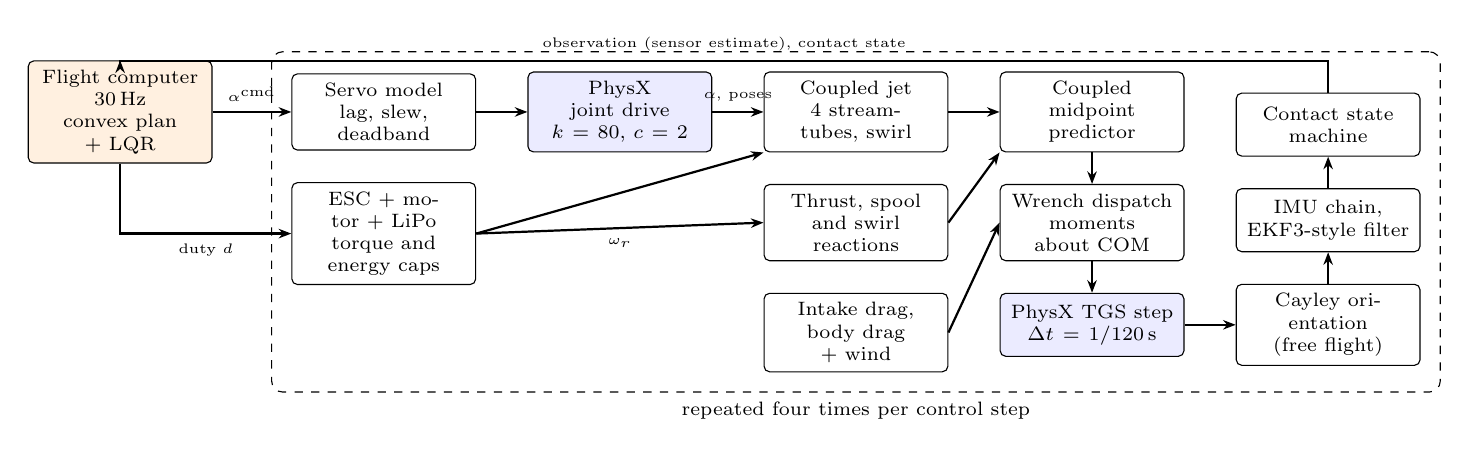
\begin{tikzpicture}[
  node distance=4mm and 6.5mm,
  box/.style={draw, rounded corners=2pt, align=center, font=\scriptsize, minimum height=8mm, text width=21mm, fill=white},
  phys/.style={box, fill=blue!8},
  ext/.style={box, fill=orange!12},
  arr/.style={-{Stealth[length=1.6mm]}, thick},
]
\node[ext] (fc) {Flight computer\\ \SI{30}{\hertz}\\ convex plan + LQR};
\node[box, right=10mm of fc] (servo) {Servo model\\ lag, slew, deadband};
\node[box, below=of servo] (motor) {ESC + motor + LiPo\\ torque and energy caps};
\node[phys, right=of servo] (drive) {PhysX joint drive\\ $k=80$, $c=2$};
\node[box, right=of drive] (jet) {Coupled jet\\ 4 streamtubes, swirl};
\node[box, below=of jet] (edf) {Thrust, spool and swirl reactions};
\node[box, below=of edf] (aero) {Intake drag,\\ body drag + wind};
\node[box, right=of jet] (pred) {Coupled midpoint predictor};
\node[box, below=of pred] (disp) {Wrench dispatch\\ moments about COM};
\node[phys, below=of disp] (physx) {PhysX TGS step\\ $\Delta t = 1/120\,\si{\second}$};
\node[box, right=of physx] (cay) {Cayley orientation\\ (free flight)};
\node[box, above=of cay] (imu) {IMU chain,\\ EKF3-style filter};
\node[box, above=of imu] (contact) {Contact state\\ machine};
\draw[arr] (fc) -- node[above, font=\tiny]{$\alpha^{\text{cmd}}$} (servo);
\draw[arr] (fc.south) |- node[pos=0.75, below, font=\tiny]{duty $d$} (motor.west);
\draw[arr] (servo) -- (drive);
\draw[arr] (drive) -- node[above, font=\tiny]{$\alpha$, poses} (jet);
\draw[arr] (motor.east) -- node[below, font=\tiny]{$\wrot$} (edf.west);
\draw[arr] (motor.east) -- (jet.south west);
\draw[arr] (jet) -- (pred);
\draw[arr] (edf.east) -- (pred.south west);
\draw[arr] (aero.east) -- (disp.west);
\draw[arr] (pred) -- (disp);
\draw[arr] (disp) -- (physx);
\draw[arr] (physx) -- (cay);
\draw[arr] (cay) -- (imu);
\draw[arr] (imu) -- (contact);
\draw[arr] (contact.north) |- ++(0,4mm) -| node[pos=0.25, above, font=\tiny]{observation (sensor estimate), contact state} (fc.north);
\begin{scope}[on background layer]
\node[draw, dashed, rounded corners, inner sep=2.5mm, fit=(servo)(motor)(drive)(jet)(edf)(aero)(pred)(disp)(physx)(cay)(imu)(contact),
      label={[font=\scriptsize]below:repeated four times per control step}] {};
\end{scope}
\end{tikzpicture}
\caption{Data flow of one control step.
Blue boxes are PhysX; white boxes are batched PyTorch models that act on PhysX through external wrenches and joint-drive targets; the flight computer reads only the simulated sensor estimate.}
\label{fig:dataflow}
\end{figure*}

\section{Propulsion, Battery and Rotor Reactions}
\label{sec:propulsion}

\subsection{Motor and ESC}
\label{sec:motor}

The ESC is modeled as a first-order speed command that a current-limited motor may or may not be able to deliver.
With $d$ the commanded duty and $V$ the loaded bus voltage, the requested acceleration and the delivered motor torque are
\begin{align}
\dot\omega_{\text{req}} &= \frac{\mathrm{clip}(d\,V/V_{\text{ref}}, 0, 1)\,\wmax - \wrot}{\tau_m}, \label{eq:esc}\\
Q_m &= \mathrm{clip}\!\left(\Ir\dot\omega_{\text{req}} + Q_a(\wrot),\; -\bar Q,\; \bar Q\right), \label{eq:motor}\\
Q_a &= \frac{P_{\max}}{\wmax}\left(\frac{\wrot}{\wmax}\right)^{2}, \nonumber
\end{align}
and the rotor obeys $\Ir\dot\omega_r = Q_m - Q_a$.
The aerodynamic torque $Q_a$ follows the momentum-theory scaling of shaft power with $\wrot^3$.
It uses the same \SI{3072}{\watt} reference as the battery load and the jet model, so the three subsystems agree on shaft power.
The motor limit $\bar Q = K_t I_{\max}$, with $K_t = 60/(2\pi\,\mathrm{KV})$, is \SI{0.76}{\newton\metre} for the planned motor at the ESC's \SI{120}{\ampere} ceiling.
EDF ESCs normally run with the brake disabled, so at $d=0$ the limit is zero and the rotor coasts down on $Q_a$.
At hover that coast has a time constant $\Ir\wrot/Q_a \approx \SI{1.7}{\second}$.
Thrust is quadratic in rotor speed, $T = k_T\wrot^2$ with $k_T = T_{\max}/\wmax^2$.

The torque limit matters physically.
Without it, the \SI{0.15}{\second} lag stopped the rotor at disarm in about \SI{0.5}{\second}.
The reaction then put \SI{5.2}{\newton\metre} on the body and spun landed vehicles at 430--\SI{710}{\degree\per\second}.
\reffig{fig:spool} compares the unbounded lag, the torque-limited motor and the full mission plant.
The bounded motor takes \SI{1.38}{\second}, rather than \SI{0.28}{\second}, to bring a cold rotor to hover speed.
It caps the spool reaction at \SI{0.76}{\newton\metre} instead of \SI{6.2}{\newton\metre}.

\begin{figure*}[t]
\centering
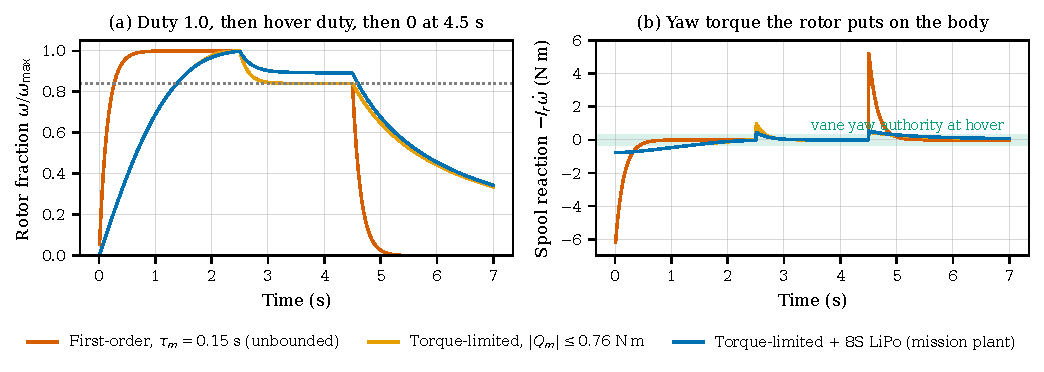
\includegraphics[width=0.9\textwidth]{spool.pdf}
\caption{Rotor response (a) and the spool reaction torque on the body (b) for a cold spool-up at full duty, a step to hover duty at \SI{2.5}{\second} and a cut to zero at \SI{4.5}{\second}, at the \SI{120}{\hertz} mission step.
The unbounded first-order lag demands up to \SI{6.2}{\newton\metre} of yaw torque, about 18 times the vanes' yaw authority at hover (shaded).
The current-limited motor bounds it, and with the brake disabled the rotor coasts after the cut.
The battery-coupled plant also follows the loaded bus voltage.}
\label{fig:spool}
\end{figure*}

\subsection{Battery Coupling}
\label{sec:battery}

The pack is a one-RC Thevenin equivalent circuit~\cite{chen2006battery,plett2015}.
The open-circuit voltage $E(\mathrm{SOC})$ is piecewise linear in state of charge, the series resistance is $R_0 = N_{\text{cell}}R_{\text{cell}}$, and $V_p$ is the polarization voltage.
For a requested electrical power
\begin{equation}
P = \frac{\left[Q_a\wrot + \tfrac{d}{dt}\!\left(\tfrac12\Ir\wrot^2\right)\right]^{+}}{\eta_m} + P_{\text{aux}},
\label{eq:power}
\end{equation}
the current is the high-voltage root of $P = I(E' - IR_0)$, $E' = E - V_p$:
\begin{equation}
I = \frac{2P}{E' + \sqrt{E'^2 - 4R_0P}}, \qquad I \le \min\!\left(I_{\max},\, \frac{E'}{2R_0}\right),
\label{eq:current}
\end{equation}
and $V = E' - IR_0$.
The bracket in \refeq{eq:power} is clamped at zero because no regenerative charging is assumed.
State of charge follows coulomb counting.
$V_p$ relaxes exactly over each step toward $IR_p$ with time constant $\tau_p$.
A lumped thermal state integrates $I^2R_0 + V_p^2/R_p$ against linear cooling.
Because the spool target depends on $V$ and the load depends on the spool, five damped fixed-point iterations resolve the pair at each substep.
When the pack cannot supply the request, the rotor may gain only the kinetic energy that the delivered shaft power provides:
\begin{equation}
\omega_r^{k+1} \le \sqrt{(\omega_r^{k})^2 + \frac{2\Delta t}{\Ir}\left(\eta_m(VI - P_{\text{aux}}) - Q_a\wrot\right)}.
\label{eq:energycap}
\end{equation}
Missions that start with a spinning rotor are placed on the loaded bus that rotor already draws.
Starting them at the open-circuit voltage made a flight computer that reads the bus voltage under-drive the rotor.
The rotor then spun down and yawed the body.

\reffig{fig:battery} shows a sustained hover on the full 8S pack.
The duty is chosen as the flight computer chooses it: by inverting the voltage-scaled speed command at the measured bus voltage.
The vehicle draws \SI{2.09}{\kilo\watt} at a rotor fraction of 0.841.
It holds hover speed for \SI{243}{\second}, until the pack can no longer sustain it at 1.2\% SOC, delivering \SI{140}{\watt\hour}.
Over that time the bus falls from 32.0 to \SI{24.4}{\volt} and the current rises from 65 to \SI{80}{\ampere}.

\begin{figure}[t]
\centering
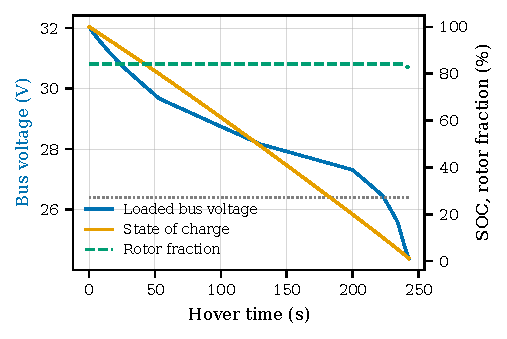
\includegraphics[width=\columnwidth]{battery.pdf}
\caption{Hover on the full 8S \SI{5}{\ampere\hour} pack, with the duty compensating the measured bus voltage.
The rotor holds hover speed until the pack can no longer supply it.
The dotted line marks \SI{3.3}{\volt} per cell.}
\label{fig:battery}
\end{figure}

\subsection{Wake, Swirl and Rotor Reactions}
\label{sec:reactions}

The ideal jet speed scales with rotor speed, $u_0 = u_{\max}\wrot/\wmax$, and the ideal wake power is $\tfrac12 T u_0$.
The stator does not recover all of the shaft torque.
The unrecovered part $Q_s = f_s P_{\max}(\wrot/\wmax)^3/\wrot$ leaves the nozzle as swirl.
Swirl kinetic power must come out of the same shaft power, so the axial speed is reduced until axial and swirl power together equal the ideal wake power:
\begin{equation}
u = \frac{u_0}{1 + Q_s^2/(T^2\langle r^2\rangle)}, \qquad \mdot = \frac{T}{u}, \qquad \Omega_s = \frac{Q_s}{\mdot\langle r^2\rangle},
\label{eq:wake}
\end{equation}
where $\langle r^2\rangle$ is the mean squared radius of the vane COPs and $\Omega_s$ the swirl rate.
At hover $\mdot = \SI{0.316}{\kilogram\per\second}$ and $u = \SI{107.5}{\metre\per\second}$.

The rotor's angular momentum $\vect{H} = \Ir\wrot\ez$ is not part of the PhysX articulation, so its reactions are applied to the body explicitly and at full strength:
\begin{equation}
\vect{\tau}_{\text{spool}} = -\Ir\dot\omega_r\,\ez, \quad
\vect{\tau}_{\text{swirl}} = -Q_s\,\ez, \quad
\vect{\tau}_{\text{gyro}} = -\wb\times\vect{H}.
\label{eq:reactions}
\end{equation}
The spool term uses the same rotor-speed step that the battery and torque limits bound.
The swirl term equals and opposes the angular-momentum flux of the swirl the vanes then see, so the motor reaction $-Q_m$, the stator recovery and the swirl close exactly.
A unit test checks this closure to \num{1e-12}.
\refsec{sec:integration} describes how the gyroscopic term is actually integrated.

The scale of these reactions explains the vehicle's character.
With $\Ir\wmax/I_{zz} = \SI{46.5}{\radian\per\second}$, every unit change in rotor fraction would spin the body by \SI{46.5}{\radian\per\second} if nothing resisted it.
The vanes can supply only \SI{0.35}{\newton\metre} of yaw torque at hover.
At hover $H = \SI{0.782}{\newton\metre\second}$, and the gyroscopic coupling $H/I_{xx} = \SI{15.6}{\radian\per\second}$ (\SI{2.49}{\hertz}) sets the frequency of the body's nutation mode.
Spinning a cold rotor up in the air hands the body about \SI{40}{\radian\per\second} of yaw.
Missions therefore spawn with the rotor already at hover speed, which represents a spool-up on the pad.

\section{Jet-Vane Aerodynamics}
\label{sec:vanes}

\subsection{From Independent Airfoils to a Shared Jet}

The original model treated each vane as an independent airfoil in the jet, $F_n = qSk_{\text{duct}}C_{N_\alpha}\alpha(1 - k_s\alpha^2)$ with $q = \tfrac12\rho u^2$.
At full rotor speed and \SI{15}{\degree} that law gives \SI{20.6}{\newton} of side force on one vane.
Yet a quarter of a \SI{48}{\newton} jet carries only \SI{12}{\newton} of axial momentum.
Turned through \SI{15}{\degree}, it can yield at most $(T/4)\sin\alpha = \SI{3.1}{\newton}$.
The airfoil law exceeds the momentum available by a factor of 6.6.

\subsection{Coupled-Jet Control-Volume Model}
\label{sec:coupledjet}

The replacement is a reduced-order control-volume model, not a blade-element fan model or CFD.
Four equal streamtubes share the mass flux $\mdot$ of \refeq{eq:wake}.
The velocity entering vane $i$, relative to the vane, is
\begin{equation}
\vect{v}_{\text{in},i} = u\,\ez + \Omega_s\ez\times\vect{r}_i^{\perp} + \wb\times\vect{r}_e - \dot{\vect{r}}_i ,
\label{eq:inflow}
\end{equation}
where $\vect{r}_i$ is the vane's measured, moving COP, $\vect{r}_i^{\perp}$ its radial part, $\vect{r}_e$ the nozzle station and $\dot{\vect{r}}_i$ the COP velocity relative to the translating body origin.
This velocity includes articulation motion.
The terms follow a frozen convected wake: the jet leaves with its nozzle's velocity, and the vane moves through it.
With $\hat{\vect{N}}_i$ the zero-deflection vane normal and $\alpha_i$ the measured deflection, the vane's actual normal and chord are
\begin{equation}
\hat{\vect{n}}_i = \hat{\vect{N}}_i\cos\alpha_i - \ez\sin\alpha_i, \qquad
\hat{\vect{c}}_i = \hat{\vect{N}}_i\sin\alpha_i + \ez\cos\alpha_i .
\label{eq:basis}
\end{equation}
The vane removes a fraction $\tau_t$ of the velocity normal to its plane, then a fraction $\delta_D$ of the velocity along its chord:
\begin{gather}
\lambda = \frac{qSk_{\text{duct}}C_{N_\alpha}}{T/4}, \qquad
\lambda_D = \frac{qSk_{\text{duct}}C_{D_0}}{T/4}, \nonumber\\
\tau_t = 1 - e^{-\lambda}, \qquad \delta_D = 1 - e^{-\lambda_D}, \nonumber\\
\vect{v}' = \vect{v}_{\text{in}} - \tau_t(\vect{v}_{\text{in}}\cdot\hat{\vect{n}})\hat{\vect{n}}, \nonumber\\
\vect{v}_{\text{out}} = \vect{v}' - \delta_D(\vect{v}'\cdot\hat{\vect{c}})\hat{\vect{c}}.
\label{eq:turning}
\end{gather}
The exponential follows from integrating $\mathrm{d}v_n/\mathrm{d}x = -k v_n$ through the vane.
At small loading it recovers the thin-airfoil slope $F_n \approx qSk_{\text{duct}}C_{N_\alpha}\alpha$.
At high loading it aligns the flow with the vane instead of reversing it.
The force on each vane is the momentum change of its streamtube, applied once at the vane's actual COP:
\begin{equation}
\vect{F}_i = \frac{\mdot}{4}\left(\vect{v}_{\text{in},i} - \vect{v}_{\text{out},i}\right).
\label{eq:vaneforce}
\end{equation}

Three properties follow by construction and are covered by unit tests.
First, the vanes are passive: $\|\vect{v}_{\text{out}}\| \le \|\vect{v}_{\text{in}}\|$, so the dissipated power $\sum_i \tfrac12(\mdot/4)(\|\vect{v}_{\text{in},i}\|^2 - \|\vect{v}_{\text{out},i}\|^2)$ is never negative.
Second, the body moment from the swirl reaction and the vanes equals the negative of the outgoing angular-momentum flux.
Third, with no jet there is no force, no reaction and no dissipation.
Induced losses follow from the turning itself and are not added a second time.
The axial component of $\sum_i\vect{F}_i$ is the vanes' thrust loss.
EDF thrust is applied raw at the body, and each vane's drag acts at its own COP, so differential drag moments are kept.
At zero deflection the vanes de-swirl the jet.
The residual swirl torque, \SI{0.047}{\newton\metre} at hover, is cancelled to \SI{2.4e-5}{\newton\metre}.
The axial loss is \SI{4.93}{\newton}, or 10.3\% of static thrust, so the net static thrust is \SI{43.1}{\newton} and the net thrust-to-weight ratio is 1.41.

\subsection{Closed Form in the Operating Regime}
\label{sec:closedform}

The loading $\lambda$ is independent of rotor speed, because $q$ and $T$ both scale with $\wrot^2$.
For the 8S parameters it is $\lambda = 7.61$, so $\tau_t = 1 - e^{-7.61} = 0.9995$.
The drag fraction is $\delta_D = 0.103$.
For a vane in an otherwise undisturbed jet, \refeq{eq:inflow}--\refeq{eq:vaneforce} then reduce exactly to a side-force magnitude of
\begin{equation}
F_{\perp} = \frac{T}{4}\left(\tau_t - \delta_D\right)\sin\alpha\cos\alpha ,
\label{eq:closed}
\end{equation}
directed against $\hat{\vect{N}}_i$, the reaction to the jet's turn.
The roll (or pitch) authority of an opposed vane pair with lever arm $\ell_z = z_v - z_c$ about the COM, and the yaw authority of a common-mode deflection at radius $r_v$, are therefore
\begin{equation}
\frac{\partial M_x}{\partial e} = \frac{T}{2}(\tau_t - \delta_D)\,\ell_z, \qquad
\frac{\partial M_z}{\partial e_c} = T(\tau_t - \delta_D)\,r_v .
\label{eq:authority}
\end{equation}
At hover ($T = \SI{33.9}{\newton}$, $\ell_z = \SI{0.11}{\metre}$, $r_v = \SI{0.04}{\metre}$) these give 1.672 and \SI{1.216}{\newton\metre\per\radian}.
The central-difference probe of the full model in the environment returns 1.672 and \SI{1.216}{\newton\metre\per\radian}.
\reffig{fig:vanes}(a) compares \refeq{eq:closed} with the model and the streamtube bound.
The residual discrepancy, below 1\%, comes from the residual swirl in the inflow.

Equation \refeq{eq:authority} has two consequences for transfer.
First, the uncertain coefficients nearly drop out.
Since $\partial\tau_t/\partial\ln C_{N_\alpha} = \lambda e^{-\lambda} \approx \num{4e-3}$, halving the lift slope lowers the authority by only 2.4\%, and doubling it raises the authority by 0.06\%.
What the model's authority does depend on is the assumption that each vane fully turns an equal quarter of the jet, together with the profile-drag fraction $\delta_D$.
Those, rather than $C_{N_\alpha}$, are what a thrust-stand vane sweep must identify.
Second, authority at hover is set by the vehicle's weight, not by the motor.
The 6S and 8S profiles give the same hover authority to four digits, because both hover at $T \approx \SI{34}{\newton}$.

\reffig{fig:vanes}(b) shows the roll authority against rotor fraction.
The authority is quadratic in rotor speed, and the airfoil model exceeds the momentum model by a factor of 8.47 at every speed.
The legacy model also carried a \SI{0.27}{\newton\metre\second\per\radian} angular damper.
Together, these made the original plant far easier to control than the vehicle it represents.

\begin{figure*}[t]
\centering
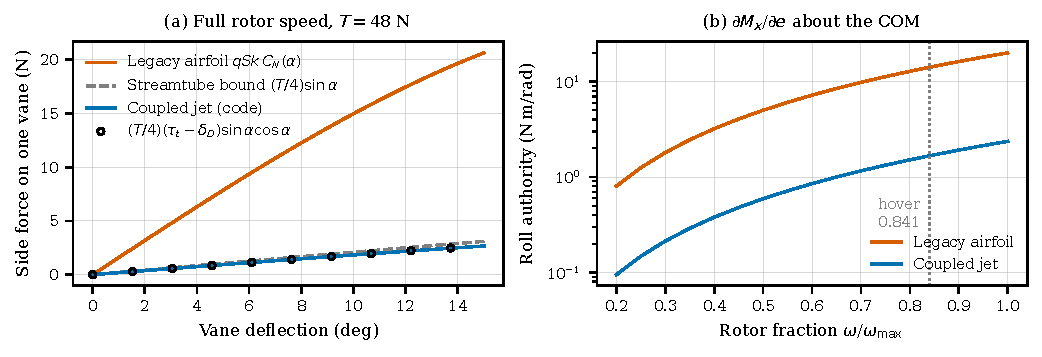
\includegraphics[width=0.9\textwidth]{vane_force.pdf}
\caption{(a) Side force on one vane at full rotor speed: the legacy independent-airfoil law, the streamtube bound $(T/4)\sin\alpha$, the coupled-jet model (de-swirl offset removed) and the closed form \refeq{eq:closed}.
(b) Roll authority about the COM against rotor fraction; the legacy law exceeds the momentum model by a factor of 8.47.}
\label{fig:vanes}
\end{figure*}

\subsection{Vane Actuation Chain}
\label{sec:servo}

The servo is a first-order lag with a slew limit and a deadband on the tracking error:
\begin{gather}
e = \begin{cases}\Delta & |\Delta| \ge b\\ 0 & \text{otherwise},\end{cases} \nonumber\\
\alpha_s^{k+1} = \mathrm{clip}\!\left(\alpha_s^{k} + \Delta t\,\mathrm{clip}\!\left(\tfrac{e}{\tau_s}, \pm\dot\alpha_{\max}\right), \pm\alpha_{\max}\right),
\label{eq:servo}
\end{gather}
with $\Delta = \alpha^{\text{cmd}} - \alpha_s$.
The explicit update is monotone, since $\Delta t/\tau_s = 0.17$.
Placing the deadband on the error rather than on the state makes the servo stop $b$ short of every command, which is backlash.
That backlash later proved to sustain a real \SI{1}{\hertz} attitude limit cycle.
A deadband inverse in the flight controller removes it~\cite{tang2026rl}.
The servo state is the target of a PhysX implicit joint drive with stiffness \SI{80}{\newton\metre\per\radian}, damping \SI{2}{\newton\metre\second\per\radian}, an effort limit at the stall torque and a velocity limit at the slew rate.
On a \SI{1}{\gram} vane the drive is overdamped, with a lag of $c/k = \SI{25}{\milli\second}$ behind the servo.
Hinge moments from the aerodynamic load act through PhysX on this drive.

The COPs move with the vanes.
At start-up each neutral metadata COP is expressed in its vane link's local frame.
Every substep it is transformed by the measured link pose, and its velocity is computed from the link's COM velocity with a COM lever arm.
Mixing a link-origin position with a COM velocity would create a spurious rotational inflow.

\section{Airframe Aerodynamics and Environment}
\label{sec:airframe}

\subsection{Translational Drag}
\label{sec:drag}

Body drag is quadratic in the air-relative velocity resolved in body axes.
Following the independence principle for slender bodies~\cite{hoerner1965}, the axial and crossflow components are separate:
\begin{equation}
\vect{F}_{\perp} = -\tfrac12\rho C_{d,\perp}A_{\perp}\|\vect{v}_{\perp}\|\vect{v}_{\perp}, \qquad
F_{\parallel} = -\tfrac12\rho C_d A_{\parallel}|v_{\parallel}|v_{\parallel},
\label{eq:bodydrag}
\end{equation}
with $\vect{v} = \vect{v}_{\text{body}} - \vect{v}_{\text{wind}}$.
The end-on area is $A_\parallel = \SI{0.011}{\metre\squared}$ and the side-on area is $A_\perp = \SI{0.042}{\metre\squared}$.
Before the most recent review, still air used the end-on area for all directions.
Enabling any disturbance file replaced it with an isotropic \SI{0.02}{\metre\squared}, so turning the wind on changed the airframe.
Drag is now taken from the vehicle geometry in calm air and in wind alike.

\subsection{Intake Momentum Drag}
\label{sec:intake}

Static thrust $k_T\wrot^2$ counts only the momentum the jet leaves with.
The intake swallows $\mdot$ of air arriving at the vehicle's air-relative velocity and turns it onto the duct axis.
That exerts the ram or momentum drag familiar from ducted-fan vehicles~\cite{johnson2006ducted,pflimlin2010ducted}:
\begin{equation}
\vect{F}_{\text{in}} = -\mdot\left(\vect{v}_{\text{rel}} + \wb\times(\vect{r}_{\text{in}} - \vect{r}_c)\right),
\label{eq:intake}
\end{equation}
applied at the intake lip $\vect{r}_{\text{in}}$, \SI{0.10}{\metre} above the COM $\vect{r}_c$.
The mass flow is the coupled jet's own.
The force reads the same wind sample as the body drag, so gusts load the intake as well.
Its power $\vect{F}_{\text{in}}\cdot\vect{v}_{\text{in}} = -\mdot\|\vect{v}_{\text{in}}\|^2$, with $\vect{v}_{\text{in}}$ the bracket in \refeq{eq:intake}, is never positive.
Along the axis it is the leading-order thrust lapse in a climb and the thrust gain in a descent.

\reffig{fig:drag} gives the crosswise force budget at hover.
Intake drag grows linearly and body drag quadratically, so they are equal at $v = 2\mdot/(\rho C_{d,\perp}A_\perp) = \SI{12.3}{\metre\per\second}$.
At \SI{1}{\metre\per\second} the intake force is 12.3 times the body's.
In a \SI{4}{\metre\per\second} wind it is \SI{1.26}{\newton}, applied with a moment of \SI{0.13}{\newton\metre} about the COM, about a third of the vanes' full-deflection authority at hover.
The plant previously omitted it entirely.
Re-flying a recorded station-keeping mission on the corrected plant changed it markedly.
The vehicle now leans \SI{5.5}{\degree} into a \SI{4}{\metre\per\second} wind and holds within \SI{0.40}{\metre}.
Before, it held within \SI{0.045}{\metre}, because the wind barely reached it.

\begin{figure}[t]
\centering
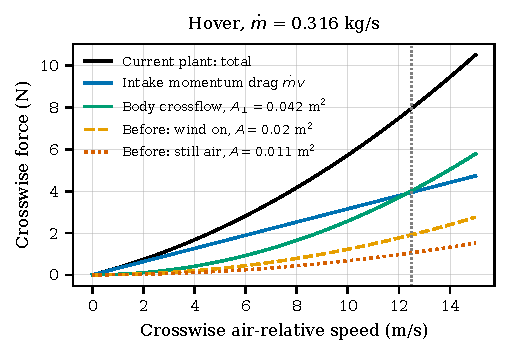
\includegraphics[width=\columnwidth]{drag.pdf}
\caption{Crosswise aerodynamic force at hover against air-relative speed.
Intake momentum drag dominates below \SI{12.3}{\metre\per\second} (dotted line).
Dashed and dotted curves show the two body-drag paths the plant used before the most recent review; neither included the intake.}
\label{fig:drag}
\end{figure}

\subsection{Rotational Damping}
\label{sec:damping}

The original simulator applied a linear angular damper of \SI{0.27}{\newton\metre\second\per\radian} that had been tuned in simulation, with no physical source.
The mission plant removes it.
What remains is physical, and \reftab{tab:damping} quantifies it by perturbing the body rate at hover in the production code.
The first term is still-air crossflow drag of a slender cylinder,
\begin{equation}
\vect{\tau}_{xy} = -\frac{\rho C_d D L^4}{64}\|\wb_{xy}\|\,\wb_{xy},
\label{eq:cyldrag}
\end{equation}
which is negligible at flight rates.
The second is vane flow damping: body rotation enters \refeq{eq:inflow} through $\wb\times\vect{r}_e - \dot{\vect{r}}_i$, and the vanes remove most of that relative flow.
The third is the rotational part of \refeq{eq:intake}, $-\mdot\,\ell_{\text{in}}^2\,\wb_\perp$.
The fourth, added in this revision, is the Coriolis reaction of the duct flow, derived below.
Together they total \SI{2.07e-3}{\newton\metre\second\per\radian} in roll and pitch.
That is 131 times less than the removed damper.
In yaw the damping is \SI{5.0e-4}{\newton\metre\second\per\radian}.

The vane-flow coefficient can be checked against Isaac.
For an axisymmetric gyrostat with transverse damping $c$, the nutation amplitude decays as $e^{-ct/I_{xx}}$.
The project's open-loop Isaac test (\reftab{tab:audit}) ran before the intake and duct terms existed and measured a decay of 0.018--\SI{0.019}{\per\second}.
The vane-flow coefficient in \reftab{tab:damping} predicts $c/I_{xx} = \SI{0.018}{\per\second}$.

\begin{table}[t]
\caption{Passive Rotational Damping at Hover (Production Code)}
\label{tab:damping}
\centering
\footnotesize
\begin{tabular}{lS[table-format=-1.2e-1]S[table-format=1.2e-1]}
\toprule
Source & {Roll/pitch} & {Yaw} \\
& {(\si{\newton\metre\second\per\radian})} & {(\si{\newton\metre\second\per\radian})} \\
\midrule
Legacy linear damper (removed) & 2.70e-1 & 2.70e-1 \\
\addlinespace
Cylinder crossflow drag at \SI{1}{\radian\per\second} & 3.45e-5 & {0} \\
Vane flow damping & 8.94e-4 & 5.05e-4 \\
Intake momentum drag, $\mdot\ell_{\text{in}}^2$ & 3.16e-3 & {0} \\
Duct Coriolis reaction \refeq{eq:coriolis} & -2.02e-3 & {0} \\
Modeled total & 2.07e-3 & 5.05e-4 \\
\bottomrule
\end{tabular}
\end{table}

\textbf{The duct Coriolis reaction.}
The intake term in \refeq{eq:intake} is only one half of the classical jet-damping bookkeeping.
Air crosses the duct from the inlet station $\vect{r}_i$ to the nozzle station $\vect{r}_e$ at a relative velocity $v_d\hat{\vect{a}}$, and a rotating vehicle must supply its Coriolis acceleration $2\wb\times v_d\hat{\vect{a}}$.
Integrating the reaction along the duct with $\mathrm{d}m = (\mdot/v_d)\,\mathrm{d}s$ gives
\begin{equation}
\vect{F}_{\text{cor}} = -2\mdot\,\wb\times(\vect{r}_e - \vect{r}_i), \quad \text{applied at } \tfrac12(\vect{r}_i + \vect{r}_e),
\label{eq:coriolis}
\end{equation}
because its moment about any point equals that of the force at the duct midpoint.
For a duct on the body axis, with stations $z_i$ and $z_e$ measured from the COM, its moment is $-\mdot(z_e^2 - z_i^2)\wb_\perp$.
Adding the intake moment $-\mdot z_i^2\wb_\perp$ gives $-\mdot z_e^2\wb_\perp$.
This is the classical jet-damping moment, which depends only on the nozzle station~\cite{thomson1986}.
The two terms also combine into a passive pair.
With $\vect{v}$ the air-relative velocity of the COM, their total power is $-\mdot\|\vect{v} + \wb\times\vect{r}_e\|^2$, so together they act like momentum drag at the nozzle.
Until this revision the simulator included the intake term alone.
With the inlet \SI{0.10}{\metre} above and the configured nozzle \SI{0.06}{\metre} below the COM, the duct reaction is \SI{-2.0e-3}{\newton\metre\second\per\radian} of damping.
Leaving it out had doubled the passive pitch and roll damping.
The mission plant now applies \refeq{eq:coriolis} beside the intake force, behind a configuration switch.
Unit tests check the integral, the classical moment and the passivity identity, and the environment's wiring through a stand-in vehicle.
The change has not yet been re-flown in Isaac.
If the effective exit were the vane plane, \SI{0.11}{\metre} below the COM, the duct reaction would add \SI{0.7e-3}{\newton\metre\second\per\radian} of damping instead, so the nozzle station should be confirmed from the CAD.
Either way the term is three orders of magnitude below the vane authority, and the closed-loop regulator, designed for zero damping, dominates it.
It does, however, set a falsifiable prediction for a free-flight test: a nutation decay of \SI{0.041}{\per\second}, against \SI{0.081}{\per\second} for the intake term alone.

\subsection{Wind, Gusts and Center-of-Mass Offset}
\label{sec:disturbances}

Wind is a steady world-frame vector plus gusts.
Each gust is a horizontal step of fixed magnitude and duration in a uniformly random azimuth.
Gusts recur after waits drawn uniformly from an interval, independently per environment.
The default disturbance uses \SI{2.0}{\metre\per\second} steady wind and \SI{5}{\metre\per\second}, \SI{0.5}{\second} gusts every 5--\SI{15}{\second}.
Missions may also draw a per-episode steady wind speed.
The center of mass may be offset per episode uniformly within \SI{\pm1}{\centi\metre} per axis.
The offset is applied to the PhysX body before the root state is written, and each new offset replaces the authored COM rather than adding to the previous one.
Because EDF thrust is applied on the airframe thrust line, an offset produces a thrust-line moment that the vanes must trim (\refsec{sec:wrench}).
Combined disturbance files retain each source's standalone strength.

\section{Rigid-Body Coupling and Numerical Integration}
\label{sec:integration}

\subsection{Wrench Application}
\label{sec:wrench}

Each vane force is applied at its moving COP, and EDF thrust, intake and body drag are applied at the authored body origin $\vect{o}$.
All moments are composed explicitly about the receiving link's actual COM $\vect{c}$:
\begin{equation}
\vect{\tau}_c = \sum_i(\vect{p}_i - \vect{c})\times\vect{F}_i + (\vect{o} - \vect{c})\times\vect{F}_b + \vect{\tau}_b ,
\label{eq:wrench}
\end{equation}
and the force and torque are passed to Isaac Lab without an application point.
The reason is two defects found in the installed Isaac Lab~2.3.2 wrench composer.
When given an application point, it crossed a world-frame lever arm with a force already rotated into link coordinates.
It also discarded any supplied torque.
Bypassing that path required no change to vendor files.
Two Isaac regressions confirm the result.
First, \SI{48}{\newton} of thrust with a \SI{\pm10}{\milli\metre} COM offset produced the expected pitch impulse to within 0.3\%.
Second, identical vane commands at four world headings produced body rates equal to within \SI{1e-7}{\radian\per\second}.

\subsection{Why Explicit Gyroscopic Integration Fails}
\label{sec:explicit}

PhysX integrates the locked-body Euler equation with an explicit treatment of $\wb\times\mat{I}\wb$.
A virtual rotor torque $-\wb\times\vect{H}$, evaluated at the old rate and applied as an external torque, is also explicit.
Linearize the torque-free gyrostat $\mat{I}\dot\wb + \wb\times(\mat{I}\wb + \vect{H}) = \vect{0}$ about a spin $r$ about the symmetry axis.
The transverse rates rotate at the nutation frequency
\begin{equation}
\omega_n = \frac{\left|(I_{zz} - I_{xx})\,r + H\right|}{I_{xx}} .
\label{eq:nutation}
\end{equation}
An explicit Euler step multiplies the transverse kinetic energy by $1 + (\omega_n\Delta t)^2$ every step.

For this vehicle the growth is large.
At hover with no body spin, $\omega_n = \SI{15.6}{\radian\per\second}$.
At \SI{120}{\hertz} the factor is 1.017 per step, which compounds to 56.9 in two seconds.
The offline replica in \reffig{fig:gyro} measures 56.93.
With the body yawing at \SI{40}{\radian\per\second} against the rotor, $\omega_n = \SI{39.6}{\radian\per\second}$, and the explicit scheme multiplies the rotational energy by \num{6.8e9} in two seconds.
At \SI{480}{\hertz} it still multiplies it by 76.
A midpoint treatment of the rotor term alone does not help when the body term dominates.
It reaches \num{1.6e8}, because the remaining explicit body term carries the instability.
The project's earliest Isaac measurements showed the same behavior.
They recorded a 10.2-fold energy gain in two unforced seconds at \SI{240}{\hertz}, and a 114-fold growth of the transverse rate squared at \SI{40}{\radian\per\second} of yaw with the rotor stopped.
Damping or a reduced gyroscopic scale would hide the error.
Neither is physical.

\subsection{Coupled Implicit Midpoint}
\label{sec:midpoint}

The mission plant therefore solves the body and rotor together with an implicit midpoint step:
\begin{equation}
\begin{split}
\mat{I}(\wb_m - \wb_k) &= \tfrac{\Delta t}{2}\left(\vect{\tau}_{\text{ext}} - \wb_m\times(\mat{I}\wb_m + \vect{H})\right),\\
\wb_{k+1} &= 2\wb_m - \wb_k ,
\end{split}
\label{eq:midpoint}
\end{equation}
where $\vect{\tau}_{\text{ext}}$ collects the vane, spool, swirl, drag and intake moments about the COM.
$\vect{H}$ uses the mean rotor speed over the step.
Four Newton iterations solve \refeq{eq:midpoint}.
The implicit midpoint rule conserves quadratic invariants, so for $\vect{\tau}_{\text{ext}} = \vect{0}$ it conserves both $\tfrac12\wb^\top\mat{I}\wb$ and $\|\mat{I}\wb + \vect{H}\|$ exactly~\cite{hairer2006}.
PhysX still supplies its own explicit term $-\wb_k\times\mat{I}\wb_k$.
The environment therefore applies the rotor torque together with an integration correction:
\begin{equation}
\vect{\tau}_{\text{gyro}} = \vect{H}\times\wb_m, \qquad
\vect{\tau}_{\text{corr}} = -\wb_m\times\mat{I}\wb_m + \wb_k\times\mat{I}\wb_k .
\label{eq:correction}
\end{equation}
With these, PhysX's explicit step lands on the midpoint solution.
The correction is an integration bridge, not damping, and it involves no target attitude.

Two further details are needed for the bridge to hold inside PhysX.
First, after its explicit update PhysX rescales the body's angular momentum to its pre-update magnitude.
The production mode inverts that projection.
It solves $\|\mat{I}(\lambda\vect{d} - \vect{b})\|^2 = \|\mat{I}\vect{d}\|^2$ for $\lambda$, with $\vect{d} = 2\wb_m - \wb_k$ and $\vect{b} = \Delta t\,\mat{I}^{-1}(-\wb_k\times\mat{I}\wb_k)$, and adds $(\lambda - 1)\mat{I}\vect{d}/\Delta t$.
Without the inversion, a case with $p = q = \SI{6.28}{\radian\per\second}$ and $r = \SI{40}{\radian\per\second}$ gained 22\% energy in two seconds at \SI{480}{\hertz}.
Second, the TGS solver must apply external forces once per step rather than at every iteration.
Re-applying a world-frame impulse while the body rotates breaks the discrete update.
The configuration loader rejects the coupled modes unless this setting is off.

\subsection{Cayley Orientation Update}
\label{sec:cayley}

PhysX advances orientation from the end-of-step rate, which is first order and inconsistent with the midpoint velocity solve.
In free flight the environment replaces that drift with the Lie-midpoint (Cayley) update paired with \refeq{eq:midpoint}:
\begin{equation}
\vect{q}_{k+1} = \vect{q}_k\otimes\mathrm{normalize}\!\left(1,\; \tfrac{\Delta t}{4}\mat{D}(\wb_k + \wb_{k+1})\right).
\label{eq:cayley}
\end{equation}
For constant $\vect{H}$ the midpoint velocity step and the Cayley rotation together conserve \emph{world} angular momentum as well as energy.
The update preserves the COM position, linear momentum and the post-solver body rates.
Whenever a contact is measured, the whole PhysX pose is left untouched, so contact impulses keep their exact effect.
\reffig{fig:gyro}(b) shows the difference.
Over two seconds at \SI{120}{\hertz}, the end-rate orientation drifts world angular momentum by \SI{0.079}{\newton\metre\second}.
The Cayley update holds it to \SI{1e-15}{\newton\metre\second}.

\begin{figure*}[t]
\centering
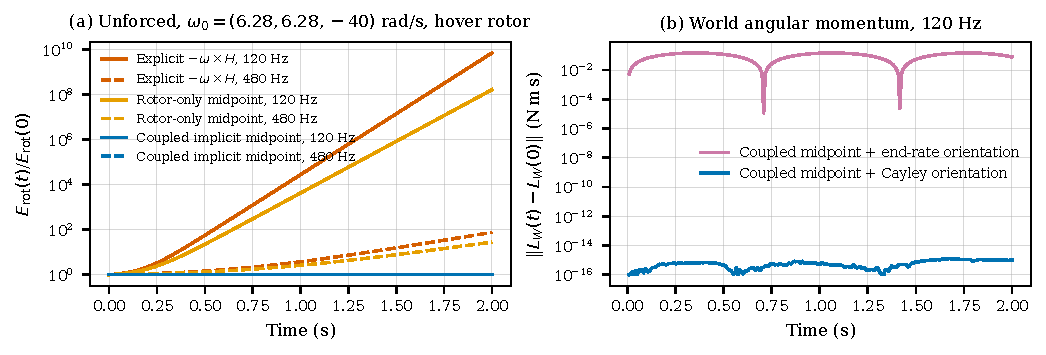
\includegraphics[width=0.9\textwidth]{gyro.pdf}
\caption{Offline replica of the integrator split for the unforced body and hover rotor, with body yaw counter to the rotor spin.
(a) Rotational energy under explicit gyroscopic torque, a rotor-only midpoint and the coupled midpoint \refeq{eq:midpoint}, at \SI{120}{\hertz} (solid) and \SI{480}{\hertz} (dashed).
(b) World angular-momentum error of the coupled midpoint paired with an end-rate orientation update or with the Cayley update \refeq{eq:cayley}.
The replica advances the locked-body term explicitly, as PhysX does, but omits PhysX's momentum projection.}
\label{fig:gyro}
\end{figure*}

\subsection{PhysX Configuration}
\label{sec:physx}

Missions use the TGS solver with four position iterations and one velocity iteration, contact and rest offsets of \SI{1}{\milli\metre} and zero, and zero PhysX linear and angular damping.
Self-collisions are disabled, and the maximum depenetration velocity is \SI{1}{\metre\per\second}.
PhysX clamps every link's angular speed to a configurable maximum and silently removes the energy above it.
Its old default of \SI{100}{\degree\per\second} was below the yaw a warm-rotor spawn alone produces, about \SI{680}{\degree\per\second}.
The default is now \SI{3600}{\degree\per\second}.
The ground is a cuboid sized automatically to the environment grid plus a \SI{150}{\metre} margin.
A fixed-size plane had left distant environments with no collider.
The ground has static and dynamic friction of 0.8 and 0.7 and a restitution of 0.05.
For parallel training, PhysX GPU buffer capacities scale with the number of environments.
Those buffers fail silently when exceeded, which shows up as missed contacts.
The Isaac plant audit (\reftab{tab:audit}) found \SI{120}{\hertz} converged against \SI{480}{\hertz} for the open-loop dynamics.

\section{Contact, Landing and Termination}
\label{sec:contact}

Landing and crash detection use PhysX contact reports on every link.
A landing contact is a normal force of at least \SI{1}{\newton} on \texttt{Body}, which carries the legs.
Any vane-link contact is unsafe.
A four-state machine, AIRBORNE, CANDIDATE, LANDED and CRASHED, requires 15 consecutive contact frames (\SI{0.125}{\second}) before LANDED.
Several rules close loopholes that earlier evaluations exposed.
\begin{itemize}
\item The recorded impact speed is the maximum downward speed at any first contact in the episode, preserved across bounces.
A later gentle re-contact cannot hide a hard first impact.
\item A crash on the final dwell frame takes precedence over a new LANDED transition.
\item The angular-rate gate is judged on arrival from flight: on the body rate before the first contact after at least one dwell of airborne frames.
Judging the rate after the contact frame flagged one-leg-first touchdowns, which pivot the body at 100--\SI{350}{\degree\per\second}, as crashes.
\item A declared ground takeoff arms the landing detector only after the vehicle climbs \SI{0.8}{\metre}.
Without this, launch support satisfies the landing dwell before the cold rotor spools.
\end{itemize}
A crash is declared for an impact faster than \SI{3}{\metre\per\second}, a tilt above \SI{0.5}{\radian} at contact, an arrival rate above \SI{3}{\radian\per\second}, or a tilt above \SI{90}{\degree}.
A successful landing requires LANDED, an impact of at most \SI{0.25}{\metre\per\second} and a pad error of at most \SI{0.5}{\metre}.
The lowest collision point lies \SI{0.3125}{\metre} below the body origin, which sets the touchdown height used by guidance.

\section{Sensor and Navigation Models}
\label{sec:sensors}

\subsection{IMU Measurement Chain}
\label{sec:imu}

Two sensor paths exist.
The legacy path adds independent white noise to the observed state at every control step.
The physical path simulates the chain a fused-attitude IMU delivers.
Specific force is $\vect{f} = \mat{R}^\top(\dot{\vect{v}} - \vect{g})$, from the velocity difference over each substep.
The sensor outputs are
\begin{align}
\vect{y}_g &= (\mat{1} + \mat{S}_g)\wb + \vect{b}_0 + \vect{k}_T\Delta T + \vect{b}_{\text{GM}} + \vect{b}_{\text{RW}} + \vect{n} + \mat{G}\vect{f}, \label{eq:gyro}\\
\vect{y}_a &= (\mat{1} + \mat{S}_a)\vect{f} + \vect{b}_0' + \vect{k}_T'\Delta T + \vect{b}_{\text{GM}}' + \vect{b}_{\text{RW}}' + \vect{n}', \nonumber
\end{align}
with scale and misalignment $\mat{S}$, turn-on bias $\vect{b}_0$, a temperature coefficient times a warm-up profile, a first-order Gauss--Markov bias, a random-walk bias, white noise and gyro $g$-sensitivity $\mat{G}$.
Every error term is redrawn per episode, so each episode is one power cycle of one randomly drawn unit.
Datasheet noise densities are one-sided amplitude spectral densities $N$, so a sample at period $\Delta t$ has variance $N^2/(2\Delta t)$.
Datasheet bias instability is read as the Allan-deviation floor.
For a Gauss--Markov process that floor is $0.6174\,\sigma$, so $\sigma_{\text{GM}} = B/0.6174$~\cite{elsheimy2008allan}.
The outputs then pass through saturation, a first-order low-pass filter with $1 - e^{-2\pi f_c\Delta t}$ gain, quantization at the output ticks, sample-and-hold at the output rate, and a transport delay of $N_d = \mathrm{round}(t_{\text{lat}}/\Delta t)$ substeps.
Each sensor model reports the rate and latency it actually delivers on the physics grid, and warns when they differ materially from the datasheet values (\refsec{sec:issues}).
The onboard attitude is a Mahony complementary filter~\cite{mahony2008}, run at the sensor rate on the measured gyro and accelerometer.
Its accelerometer correction is gated on $\big|\|\vect{y}_a\| - g\big|$.
Yaw is gyro-only, or optionally magnetometer-aided.
Three profiles are provided: WTGAHRS1, BNO085 and VN-110E.
Each parameter is tagged as datasheet, manual, estimate or placeholder.
The gyro's true input can be derived from the pose change rather than from PhysX's reported rate.
During pad contact PhysX corrects the pose without a matching angular velocity.
A gyro integrating the reported rate carried a \SI{0.8}{\degree} pitch error from the first touchdown, which dead reckoning turned into \SI{6}{\metre} of drift in \SI{10}{\second}.

\reffig{fig:imu} illustrates two consequences, using the production chain driven by scripted kinematics at the mission step.
In panel (a), most of the gyro error on a fast-changing rate is lag, not noise.
On a \SI{1.07}{\hertz}, \SI{15}{\degree\per\second} roll oscillation the WTGAHRS1 profile delivers \SI{0.92}{\degree\per\second} RMS error on a \SI{10.7}{\degree\per\second} RMS signal.
A white-noise model cannot represent that.
In panel (b), on a thrust-vectored vehicle the accelerometer always reads along the body axis.
Accelerometer aiding therefore drags the tilt estimate toward level during a sustained banked acceleration.
With the profiles' filter gains the error reaches 7.7, 7.9 and \SI{4.4}{\degree} after \SI{10}{\second} of a \SI{10}{\degree} bank for the WTGAHRS1, BNO085 and VN-110E.
No single gain is good.
Low gains leave the gyro bias uncorrected, and high gains follow the thrust vector.

\begin{figure*}[t]
\centering
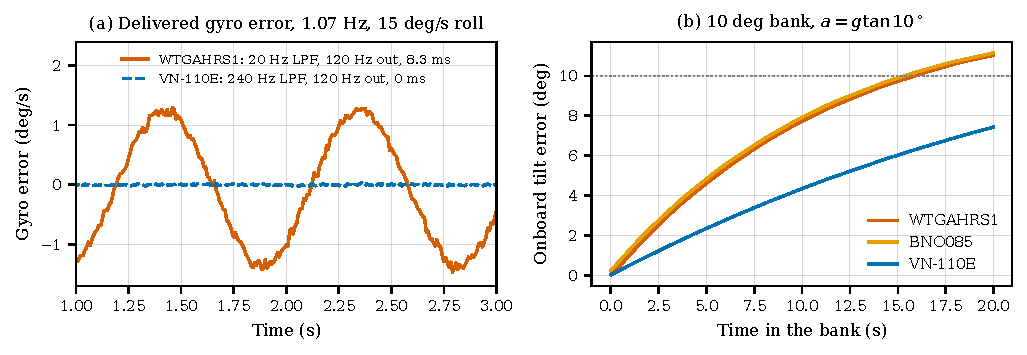
\includegraphics[width=0.9\textwidth]{imu.pdf}
\caption{Production IMU chain at the \SI{120}{\hertz} mission step with scripted kinematics.
(a) Gyro error during a \SI{1.07}{\hertz} roll oscillation; legends give the effective filter bandwidth, output rate and latency at this step.
(b) Onboard tilt error during a sustained \SI{10}{\degree} bank with the consistent acceleration $g\tan\SI{10}{\degree}$.}
\label{fig:imu}
\end{figure*}

\subsection{Aiding Sensors and Navigation Filter}
\label{sec:nav}

An optional fused path adds three downward and onboard sensors: a Benewake TFmini Plus rangefinder, a MicoAir MTF-01P optical-flow sensor and a barometer.
The rangefinder reads the slant range $r = h/\cos\theta - d_{\text{mount}}$.
The flow sensor reads the apparent ground rate $\vect{f} = (v_{s,y}/r - \omega_x,\, -v_{s,x}/r - \omega_y)$.
The barometer reads height with a slow Gauss--Markov drift.
Each sensor samples physics truth at its own rate, corrupts it, holds it for its latency, and reports its age in substeps.
A 16-state error-state EKF fuses them with the IMU's raw registers~\cite{sola2017}.
Its states are attitude error, velocity, position, gyro bias, accelerometer bias and terrain height.
It follows ArduPilot EKF3's structure and default noise and gate parameters~\cite{ardupilot2026ekf3}.
Late measurements are compared with the stored state at their sample time, and the correction is applied to the current state.
An optional downward camera on a fiducial marker at the pad supplies the only absolute horizontal reference, between 0.3 and \SI{8}{\metre} of estimated height.
Truth remains physics truth for scoring.
A vehicle navigating on a drifting estimate visibly misses the pad.
The project's recorded hover-and-land missions show what this path provides.
Flow-only fused navigation lands softly but 1.4--\SI{1.7}{\metre} from the pad, and adding the marker reduces that to \SI{0.07}{\metre}.
Unaided dead reckoning drifted 7--\SI{130}{\metre} on the same flight.

\section{Convex Powered-Descent Guidance and Flight Control}
\label{sec:guidance}

The simulator exists to develop a controller that can transfer to the vehicle.
That controller is explicit convex guidance.
A second-order cone program (SOCP) plans the thrust trajectory from the current state to the pad, and the plan is re-solved in closed loop.
A tracking loop, a gyroscopic attitude regulator and a throttle model realize it on the vanes and the rotor.
This section describes the planner and the flight controller as implemented (\texttt{convex\_guidance.py}, \texttt{convex\_adapter.py}, \texttt{attitude\_lqr.py}).
It emphasizes how each constraint follows from the physics of \refsec{sec:propulsion}--\refsec{sec:integration}.
The controller reads only the simulated sensor estimate, the mission route and the measured bus voltage.
It never reads simulator truth.

\subsection{Constraints Derived from the Plant}
\label{sec:limits}

The planner's bounds are not tuning constants.
At every re-plan the flight computer derives them from the vehicle model it holds, which the mission runner builds from the plant itself.
That model contains the mass, the level-hover rotor fraction, the probed vane authorities $K = \SI{2.365}{\newton\metre\per\radian}$ (roll and pitch) and $K_{\psi} = \SI{1.720}{\newton\metre\per\radian}$ (yaw) at full rotor speed, the rotor momentum $\Ir\wmax$, the inertias and the actuator lags.
\reftab{tab:limits} lists the results for the 8S plant.

The thrust ceiling keeps half of the thrust above weight in reserve for the tracking loop:
\begin{equation}
\rho_2 = W + (1 - r)\left(T_{\text{av}}(V) - W\right), \qquad r = 0.5,
\label{eq:rho2}
\end{equation}
where $T_{\text{av}}(V) = T_{\text{full}}\min(1, V/V_{\text{ref}})^2$ falls as the pack sags.
The floor $\rho_1$ is positive for two reasons.
The vanes need jet flow for authority, so $\rho_1 \ge 0.6\,W$.
Also, a plan may not accelerate downward harder than it can brake, $W - \rho_1 \le \rho_2 - W$.
The second condition sets $\rho_1 = 0.79\,W$ on the 8S plant.

Three rate bounds come from the rotor's angular momentum.
A duty slew $\dot d$ changes rotor speed at $\wmax(V/V_{\text{ref}})\dot d$, and its reaction torque about the thrust axis can be held only by the vanes' common mode.
The duty slew is therefore bounded so that this reaction uses at most 40\% of the yaw torque available at hover:
\begin{equation}
\Ir\wmax\frac{V}{V_{\text{ref}}}\,\dot d \le 0.4\,\min\!\left(K_\psi f_h^2\delta_{\max},\ \tau_{\psi}\right),
\label{eq:dutyrate}
\end{equation}
where $f_h$ is the hover rotor fraction, $\delta_{\max}$ the vane effort limit and $\tau_\psi = \SI{0.3}{\newton\metre}$ the yaw loop's design torque.
Through $T = T_{\text{full}}(d V/V_{\text{ref}})^2$, this becomes a thrust-rate bound $\dot T \le 2\sqrt{T T_{\text{full}}}\,(V/V_{\text{ref}})\,\dot d$, evaluated at the lowest planned thrust.
Tilting the body at a rate $\omega_t$ precesses the rotor and takes a vane torque $H\omega_t$.
The planned attitude slew is therefore limited to 40\% of the slew that full vane deflection can sustain at hover:
\begin{equation}
\omega_t \le 0.4\,\frac{K f_h^2\delta_{\max}}{\Ir\wmax f_h} .
\label{eq:tiltrate}
\end{equation}
The remaining 60\% of vane authority is left for disturbance rejection.
The same expression with a 0.6 share bounds the body-rate command of the attitude loop.
The vane-yaw reserve, the common-mode travel that holds the rotor reaction at the bounded duty slew, is kept free for yaw in the mixer.

\begin{table}[t]
\caption{Guidance Limits Derived from the 8S Plant at a \SI{32}{\volt} Bus}
\label{tab:limits}
\centering
\footnotesize
\setlength{\tabcolsep}{3pt}
\begin{tabular}{>{\raggedright\arraybackslash}p{0.33\columnwidth}>{\raggedright\arraybackslash}p{0.27\columnwidth}>{\raggedright\arraybackslash}p{0.32\columnwidth}}
\toprule
Quantity & Value & Origin \\
\midrule
Floor $\rho_1$ & \SI{24.14}{\newton} (0.79\,$W$) & braking symmetry, $\ge 0.6\,W$ \\
Weight $W$ & \SI{30.45}{\newton} & \\
Ceiling $\rho_2$ & \SI{36.76}{\newton} (1.21\,$W$) & \refeq{eq:rho2}, $T_{\text{av}} = \SI{43.07}{\newton}$ \\
Duty slew & \SI{0.119}{\per\second} & \refeq{eq:dutyrate} \\
Thrust rate & \SI{7.19}{\newton\per\second} & at $0.6\,W$ \\
Planned attitude slew & \SI{12.0}{\degree\per\second} & \refeq{eq:tiltrate} \\
Attitude-loop rate command & \SI{18.0}{\degree\per\second} & \refeq{eq:tiltrate}, share 0.6 \\
Yaw reserve & \SI{0.098}{\radian} of \SI{0.245}{\radian} & rotor reaction at the duty slew \\
Emergency thrust rate & \SI{243}{\newton\per\second} & spool-up slew \SI{4}{\per\second} \\
Sink-envelope deceleration & \SI{0.71}{\metre\per\second\squared} & $0.35(\rho_2/m - g)$ \\
\addlinespace
Pointing, glide slope & \SI{15}{\degree}, \SI{45}{\degree} & configuration \\
Speed bound & \SI{4}{\metre\per\second} & configuration \\
Gate & \SI{0.5}{\metre} up, \SI{0.15}{\metre\per\second} & above touchdown height \\
\bottomrule
\end{tabular}
\end{table}

\subsection{Planning Model and Discretization}
\label{sec:plannermodel}

The planner treats the vehicle as a constant-mass point with thrust acceleration $\vect{u} = \vect{T}/m$, $\ddot{\vect{r}} = \vect{u} + \vect{g}$.
A battery vehicle loses no mass, so the logarithmic mass variable of the original method is unnecessary and the problem is an exact SOCP.
The thrust is a first-order hold: linear between $N + 1$ nodes rather than piecewise constant.
The dynamics are integrated exactly over each interval:
\begin{equation}
\begin{split}
\vect{r}_{k+1} &= \vect{r}_k + \Delta t\,\vect{v}_k + \Delta t^2\left(\tfrac13\vect{u}_k + \tfrac16\vect{u}_{k+1} + \tfrac12\vect{g}\right),\\
\vect{v}_{k+1} &= \vect{v}_k + \Delta t\left(\tfrac12(\vect{u}_k + \vect{u}_{k+1}) + \vect{g}\right).
\end{split}
\label{eq:foh}
\end{equation}
The first node's thrust is fixed to the rotor's present thrust vector, its magnitude from rotor speed and its direction from the body axis.
Because the thrust is continuous, the rate bound below bounds the thrust the vehicle actually has to follow.
A zero-order hold stepped the thrust direction at every node.
On a recorded \SI{30}{\metre} approach, those steps reached \SI{8.6}{\degree} every \SI{0.46}{\second}, which the rate-limited rotor and the precession-limited attitude loop cannot follow.
The landing leg uses 24 intervals.
Waypoint legs use about \SI{0.35}{\second} intervals and at most 40 per leg.
The plan is sampled exactly, as a cubic in position, by the tracking loop.

\subsection{Lossless Convexification}
\label{sec:lcvx}

The thrust annulus $\rho_1 \le \|\vect{T}\| \le \rho_2$ is non-convex.
Following A\c{c}{\i}kme\c{s}e and Ploen~\cite{acikmese2007}, it is relaxed with a slack $\sigma_k$:
\begin{equation}
\|\vect{u}_k\| \le \sigma_k, \qquad \rho_1/m \le \sigma_k \le \rho_2/m ,
\label{eq:lcvx}
\end{equation}
and the thrust-pointing constraint is written on the slack, $u_{z,k} \ge \sigma_k\cos\theta_{\max}$.
For costs that increase with $\sigma$, the relaxation is lossless under the method's conditions~\cite{acikmese2007,acikmese2011lcvx}.
At the optimum $\|\vect{u}_k\| = \sigma_k$, so the planned thrust respects the annulus.
Every plan reports the gap $\max_k(\sigma_k - \|\vect{u}_k\|)/\sigma_k$, so losslessness is checked numerically rather than assumed.

The vehicle-specific constraints leave the hypotheses of that result.
The thrust-rate bound couples successive controls, which makes thrust effectively a state.
State constraints are known to break the guarantee in general~\cite{harris2014lcvx}.
With the production limits, plans from offset starts are lossless to round-off, with gaps of \num{1.4e-9} to \num{2.2e-9}.
A near-vertical entry descending at \SI{1}{\metre\per\second} from \SI{18}{\metre} is not.
There the energy-optimal plan ramps thrust down at the rate bound, and for two nodes it uses the slack to place $\|\vect{u}\|$ below $\sigma = \rho_1/m$.
The planned thrust reaches \SI{23.4}{\newton} against a \SI{24.1}{\newton} floor, a gap of 3.2\%.
The dip remains well above the \SI{18.3}{\newton} authority floor, because $\rho_1$ is set here by braking symmetry rather than by authority, so the effect was benign.
It does show that the gap must be monitored rather than assumed zero.
The project's unit tests had asserted a small gap only under a different set of limits.

This revision therefore adds a two-level safeguard.
Within one fixed-duration solve, nodes whose gap exceeds \num{1e-3} receive the convex half-space floor $\vect{u}_k\cdot\hat{\vect{d}}_k \ge \rho_{1,k}/m$ along their solved thrust direction $\hat{\vect{d}}_k$.
This floor implies $\|\vect{u}_k\| \ge \rho_{1,k}/m$, and the problem is solved once more.
In the duration search, a plan that is still gapped counts as infeasible, and it is kept only if no duration yields a lossless plan.
Such gaps sit at the short, minimum-energy edge of feasibility (\refsec{sec:freetime}), where the floored problem is often infeasible, so the search moves to a slightly longer duration.
For the near-vertical entry the plan becomes lossless (gap \num{2.4e-9}), with a thrust of at least \SI{25.0}{\newton}.
It lasts \SI{8.05}{\second} instead of \SI{7.87}{\second} and costs 2\% more energy.
Plans that were already lossless never trigger the safeguard and are bit-identical to before.
A regression test reproduces the gap with the mission plant's limits and checks both properties.

\subsection{Constraints}
\label{sec:constraints}

All constraints are convex and imposed at the nodes.
\begin{itemize}
\item \textbf{Thrust rate.} $\|\vect{u}_{k+1} - \vect{u}_k\| \le \dot T_{\max}\Delta t/m$ on the thrust \emph{vector}.
A bound on the slack would not bound $\|\vect{u}\|$ once $\sigma > \|\vect{u}\|$.
The vector form also bounds the thrust-direction slew.
\item \textbf{Attitude slew.} $\|\vect{u}_{xy,k+1} - \vect{u}_{xy,k}\| \le g\,\omega_t\Delta t$, which bounds the tilt rate to first order in tilt.
\item \textbf{Glide slope.} $\|\vect{r}_{xy,k} - \vect{a}_{xy}\| \le \tan\gamma_k\,(z_k - a_z)$ with the apex $\vect{a}$ at touchdown.
A start outside the \SI{45}{\degree} cone gets a widened cone that narrows linearly back to nominal \SI{3}{\second} before the gate.
Widened for the whole leg, every re-plan rode the wide cone, and the vehicle reached the gate still moving sideways.
\item \textbf{Speed.} $\|\vect{v}_k\| \le \max\!\left(V_{\max},\ v_e - b\,(t_k - t_s)^+\right)$.
A fast entry keeps its speed $v_e$ while the rate-limited thrust settles over $t_s$, then brakes back under $V_{\max}$ at half the slowest braking the limits allow.
A single cap based on $\|\vect{v}_0\|$ let each re-plan fly faster than the last, ratcheting the speed from 4.0 to \SI{5.9}{\metre\per\second} on a recorded approach.
\item \textbf{Sink-rate envelope.} On the landing leg,
\begin{equation}
-v_{z,k} \le s_k, \qquad s_k^2 \le v_g^2 + 2a\,(z_k - z_g),
\label{eq:sink}
\end{equation}
a rotated second-order cone, written as $\|(2s_k,\, L_k - 1)\| \le L_k + 1$ with $L_k$ the right-hand side.
From every node the vehicle can still brake to the gate speed $v_g$ using $a = 0.35(\rho_2/m - g)$, a third of its planned braking capacity.
Without the envelope, an energy-optimal leg from a \SI{4.6}{\metre} hover sank at \SI{2.0}{\metre\per\second} and braked on the thrust-rate bound.
That bound is the whole yaw-safe duty slew, so the tracking loop had no slew left to make up the rotor's lag, and two recorded missions touched down at 1.7 and \SI{2.1}{\metre\per\second}.
\item \textbf{Gate.} The plan ends at a gate \SI{0.5}{\metre} above touchdown height, descending vertically at \SI{0.15}{\metre\per\second}.
Its final thrust is vertical and equals weight, $\vect{u}_N = (0, 0, g)$, so the hand-over to the terminal descent needs no thrust step.
Landing-leg nodes stay at or above the gate altitude, so the plan cannot dip under the gate and climb back.
\item \textbf{Routes.} A fly-through waypoint constrains a node to a capture ball and its velocity to the leg speed along the route tangent, or optionally to a cone around the tangent.
A hover waypoint fixes position, zero velocity and hover thrust, and holds them for the remaining dwell.
An optional soft corridor keeps each node within a half-width of the drawn Catmull--Rom route, measured as the convex distance to a chord, with the excess priced in the cost.
\end{itemize}

\subsection{Objective}
\label{sec:objective}

The primary objective is electrical energy.
The plant's power law is $P(T) = (P_{\max}/\eta_m)(T/T_{\text{full}})^{3/2} + P_{\text{aux}}$, the same momentum-theory scaling as \refeq{eq:motor}.
Each node gets an epigraph variable $c_k \ge \sigma_k^{3/2}$, expressed as the power cone $(c_k, 1, \sigma_k) \in \mathcal{K}_{\text{pow}}(2/3)$, and the nodes are combined with trapezoid weights $w_k$:
\begin{equation}
\min\ \sum_k w_k c_k + J_{\text{sec}}, \qquad c_k^{2/3}\cdot 1^{1/3} \ge \sigma_k .
\label{eq:energy}
\end{equation}
A propulsive delta-v objective, $\sum_k w_k\sigma_k$ (the method's fuel analog), is the alternative.
The optional secondary terms $J_{\text{sec}}$ are all priced in seconds of hover cost.
They are cross-track distance from the drawn route, plan duration, squared thrust jerk and squared horizontal thrust.
The quadratic terms make the problem a QP--SOCP.
None of them involves $\sigma$, so they do not affect the losslessness argument.
All of them are off in the repository defaults that the reported missions flew.

\subsection{Free Final Time and Fallback}
\label{sec:freetime}

The landing duration is free.
As in the original method's Algorithm~1, it is found by a one-dimensional search over fixed-duration SOCPs.
Without a previous plan, the search samples eight durations geometrically between bounds set by the distance and speed limit.
When re-planning, it samples three durations around the previous plan's remaining time.
Golden-section refinement~\cite{kiefer1953} then follows.
The independent problems are solved in parallel on four threads.
\reffig{fig:search} shows the cost against duration for the plan of \reffig{fig:plan}.
Short durations are infeasible, and beyond the feasibility boundary the cost rises almost linearly, at about \SI{0.58}{\watt\hour\per\second}, the hover power.
For this vehicle, hover power dominates, so the energy-optimal duration sits at the edge of feasibility.
The plan therefore rides its rate, speed and envelope bounds, and the margins come only from the explicit reserves in \reftab{tab:limits}.
The search stops \SI{0.04}{\second} short of the boundary, which costs 0.5\% energy.

If no duration is feasible, for example after a start too fast and too low to stop, a soft-terminal problem minimizes the weighted miss of the gate position and velocity.
It keeps every actuator constraint, drops the state constraints and treats ground clearance as a heavily penalized constraint.
It may also use the full available thrust and the spool-up slew.
The plan therefore degrades to maximum braking rather than to no plan.
On a route the soft target is the active waypoint, never the pad, so waypoints are not skipped.

Problems are solved with Clarabel~0.11, a primal-dual interior-point conic solver~\cite{goulart2024clarabel}, with a \SI{0.5}{\second} limit per SOCP.
On an Apple M1 Max a landing plan takes 15 SOCPs of 24 nodes and 61--\SI{71}{\milli\second} in total.
The selected solve converges in 15--20 interior-point iterations.
The project measured \SI{48}{\milli\second} mean and \SI{74}{\milli\second} maximum per landing plan on a Ryzen~9 9900X, and estimates that a Raspberry Pi~5 or Jetson Orin Nano CPU is four to five times slower.

\begin{figure*}[t]
\centering
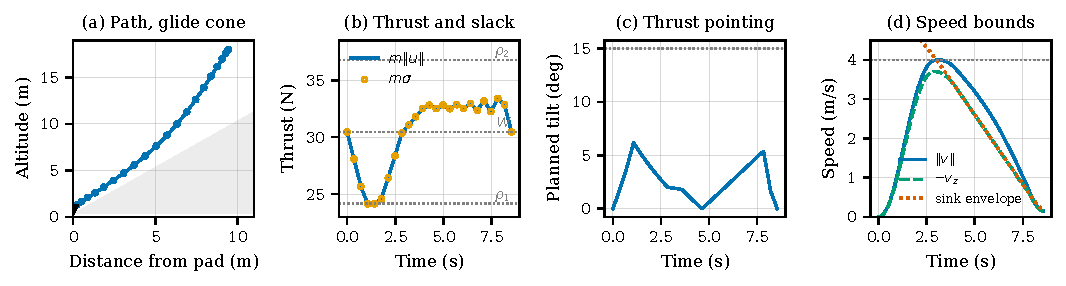
\includegraphics[width=\textwidth]{convex_plan.pdf}
\caption{Energy-optimal landing plan from $(8, 5, 18)$\,\si{\metre} at rest, solved by the production planner with the limits of \reftab{tab:limits}.
(a) Horizontal distance against altitude; the shaded region is excluded by the \SI{45}{\degree} glide cone, and the triangle marks the gate.
(b) Planned thrust $m\|\vect{u}\|$ and slack $m\sigma$ (nodes), coincident because the relaxation is lossless here; dotted lines mark $\rho_1$, $W$ and $\rho_2$.
(c) Planned tilt against the \SI{15}{\degree} cone.
(d) Speed against the \SI{4}{\metre\per\second} bound, and sink rate against the envelope \refeq{eq:sink}.}
\label{fig:plan}
\end{figure*}

\begin{figure}[t]
\centering
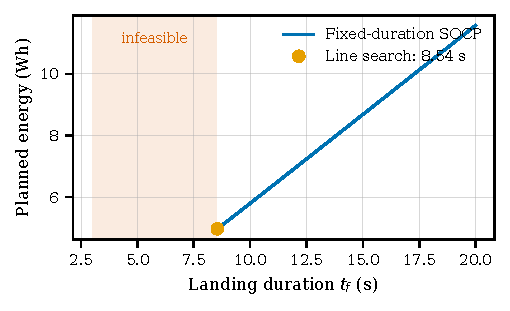
\includegraphics[width=\columnwidth]{convex_search.pdf}
\caption{Planned energy of the fixed-duration SOCP against landing duration for the plan of \reffig{fig:plan}.
Durations below \SI{8.5}{\second} are infeasible; the line search returns \SI{8.54}{\second}.}
\label{fig:search}
\end{figure}

\reffig{fig:plan} shows a representative plan.
It descends along the speed bound, tilts by at most \SI{6.2}{\degree}, slews at up to \SI{11.3}{\degree\per\second} against the \SI{12.0}{\degree\per\second} bound, and brakes along the sink-rate envelope to the gate.
Its thrust rate reaches the \SI{7.19}{\newton\per\second} bound during the initial ramp-down.
One artifact is visible in panel (b).
While the envelope binds, the planned thrust alternates by up to \SI{\pm0.5}{\newton} from node to node.
The constraints hold only at the nodes, and the first-order hold lets alternating thrusts satisfy them there.
The tracking loop's thrust lead and the rotor's rate limit filter the alternation.
The smoothness term of \refsec{sec:objective} would remove it.

\subsection{Closed-Loop Execution}
\label{sec:closedloop}

The flight computer re-solves every \SI{0.5}{\second}, when the route changes, or when the tracking error exceeds \SI{0.75}{\metre}.
While the vehicle tracks within \SI{0.75}{\metre} and \SI{0.75}{\metre\per\second} of the plan, the new plan starts from the old plan's reference state, so feedback keeps working on the deviation.
Re-solving from the measured state every period zeroed the tracking error each time.
Each new plan then started wherever the vehicle had drifted, and in a recorded mission the vehicle orbited the pad.
Larger deviations re-plan from the measured state.
Re-planning stops in the final \SI{0.8}{\second} before the gate.
After each re-plan the thrust feedforward cross-fades from the replaced plan over \SI{0.3}{\second}, because each new plan starts at the present thrust but with its own slope.
A deployment model makes planning latency explicit: a re-plan requested at time $t$ replaces the tracked plan only at $t + t_{\text{plan}}$, with its clock starting at $t$.
On the flight computer the solve runs in a separate process beside the \SI{30}{\hertz} loop.
In offline replicas, landings stay soft with up to \SI{1}{\second} of latency.

The controller moves through five phases.
\begin{itemize}
\item \textbf{SPOOL\_UP.} With a cold rotor below the thrust floor, the controller holds level and ramps the duty to hover at \SI{4}{\per\second}.
\item \textbf{POWERED\_DESCENT} or \textbf{ROUTE.} The controller tracks the plan.
\item \textbf{TERMINAL\_DESCENT.} From the gate, the controller flies a velocity-commanded vertical descent at \SI{0.15}{\metre\per\second}, clamped at \SI{0.18}{\metre\per\second}.
The descent pauses while the vehicle is more than \SI{0.2}{\metre} off center, except below a \SI{0.15}{\metre} commit height.
A contact candidate latches a land detector that levels the body and unloads the rotor to half of weight, so the contact dwell of \refsec{sec:contact} completes.
\item \textbf{HOLD.} With no feasible plan yet, the controller holds position.
\end{itemize}
A braking monitor integrates the fastest stop the yaw-safe duty slew allows.
If that stop needs more than 85\% of the height above touchdown, the duty slews at the spool-up rate instead, trading a yaw transient for braking, as the soft-terminal fallback does.

\subsection{Tracking and Thrust Realization}
\label{sec:tracking}

The plan's thrust acceleration, sampled one spool lag (\SI{0.15}{\second}) ahead, is the feedforward.
World-frame PID feedback corrects it:
\begin{equation}
\vect{a}_{\text{cmd}} = \vect{u}_{\text{ff}}(t + t_{\text{lead}}) + \mat{K}_p\vect{e}_r + \mat{K}_d\vect{e}_v + \mat{K}_i\!\int\mathrm{sat}(\vect{e}_r)\,\mathrm{d}t .
\label{eq:track}
\end{equation}
The gains are 1.0, 1.2 and 0.3 horizontally and 1.5, 2.5 and 0.3 vertically.
The integrators absorb thrust-model bias, wind and the side force of a COM trim.
Each integrator is bounded by the acceleration it may command, \SI{1.5}{\metre\per\second\squared}.
It integrates only near steady flight, and the error it integrates saturates at \SI{0.5}{\metre}.
Otherwise it would learn manoeuvre lag and carry it into the terminal phase as a bias.
The commanded thrust $m\vect{a}_{\text{cmd}}$ is limited to a \SI{22}{\degree} cone and to $[0.5\,W, T_{\text{av}}]$.
Its direction is the desired body axis.
Its component along the actual body axis sets the duty by inverting the battery-coupled speed law, $d = \sqrt{T/T_{\text{full}}}\,V_{\text{ref}}/V$, at the measured bus voltage.
The duty is slewed at the rate \refeq{eq:dutyrate}, applied to the rotor command $dV/V_{\text{ref}}$ rather than to the raw duty.
A duty change that only compensates a bus-voltage change therefore passes at once.
Slewing the raw duty had held that compensation back on warm starts, spinning the rotor down and yawing the body.

The lateral loop has a subtlety specific to jet vanes.
The vanes push the vehicle sideways directly, at about \SI{59}{\metre\per\second\squared} per radian of effort.
That push opposes the tilt they command, which makes the lateral response non-minimum-phase.
A linear hover model of the complete loop shows that this side force caps the usable velocity gain.
At $k_d = 1.2$ the loop is damped at $\zeta = 0.37$; at 1.6 the damping falls to 0.03 when the whole feedback correction is fed forward into the attitude loop.

\subsection{Gyroscopic Attitude Regulation}
\label{sec:lqr}

The attitude error is geometric, $\vect{e} = \tfrac12(\mat{R}_d^\top\mat{R} - \mat{R}^\top\mat{R}_d)^\vee$~\cite{lee2010geometric}.
$\mat{R}_d$ keeps the current heading, because heading is free for this axisymmetric vehicle.
The rotor's momentum dominates roll and pitch:
\begin{equation}
\begin{split}
I\dot p &= Kf^2 j_x - Hq - cp, \qquad I\dot q = Kf^2 j_y + Hp - cq,\\
\dot s &= (u - s)/\tau_s, \qquad \dot j = (s - j)/\tau_j ,
\end{split}
\label{eq:attplant}
\end{equation}
where $H = \Ir\wmax f$, $s$ is the servo angle and $j$ the vane-joint angle in effort space, and the lags are $\tau_s = \SI{0.05}{\second}$ and $\tau_j = \SI{25}{\milli\second}$ (\refsec{sec:servo}).
A torque about one axis mostly precesses the body about the other.
The unforced motion is the nutation at $H/I \approx \SI{2.5}{\hertz}$ (\reftab{tab:audit}), where the vane actuators lag about \SI{0.075}{\second}.
Rate feedback passes \SI{90}{\degree} of phase there and stops damping.
\reffig{fig:lqr} shows the result for the mission's earlier proportional-derivative law.
On the momentum-vane plant it is linearly unstable above a rotor fraction of 0.67, which covers the whole flight range.
At hover it has a \SI{4.1}{\hertz} nutation mode growing at \SI{1.68}{\per\second} and a \SI{1.6}{\hertz} mode growing at \SI{1.05}{\per\second}.
On the legacy plant, the \SI{0.27}{\newton\metre\second\per\radian} damper had masked this instability.
On the momentum plant, only saturation and the servo deadband bounded it, as the limit cycles observed in Isaac.

The replacement is a discrete LQR on the full state of \refeq{eq:attplant}.
The state is $\vect{x} = [\int\vect{e},\, \vect{e},\, \vect{\omega}_{xy} - \vect{\omega}_{\text{ref}},\, \vect{s} - \vect{s}_h,\, \vect{j} - \vect{j}_h]$, ten states for roll and pitch.
Both actuator states are measurable: the joint state is the measured vane angle, and the servo state is $j + \tau_j\dot j$.
They supply the phase lead a PD law lacks.
The gains solve the discrete algebraic Riccati equation for the zero-order-hold model at \SI{30}{\hertz}, with diagonal weights of 3000, 1000 and 30 on the error integral, the error and the rates.
The input is weighted by Bryson's rule~\cite{bryson1975} on vane torque, $R = (\SI{0.24}{\newton\metre})^{-2}K^2$ per unit effort.
The design is therefore the same torque loop on any vanes; weighting the effort itself made the design 72 times more aggressive on the legacy vanes.
The gains are scheduled on rotor fraction from 0.3 to 1.0, because both $Kf^2$ and $H$ change with it.
At hover the slowest closed-loop modes decay at 1.92 (the trim integral) and \SI{3.96}{\per\second}.
The smallest damping ratio of an oscillatory mode is 0.46 at hover and 0.40 over the whole range.
The project's robustness checks keep $\zeta \ge 0.24$ under $\pm30\%$ authority, $+50\%$ actuator lag, \SI{8}{\milli\second} of extra delay, $\pm20\%$ inertia or $+20\%$ rotor momentum, applied one at a time.

Yaw is a separate channel on $[\int r,\, r,\, s,\, j]$ with the same actuator model.
Its integral term cancels the steady \SI{0.05}{\newton\metre} residual-swirl torque, which rate feedback alone left as a 15--\SI{27}{\degree\per\second} spin.
To follow a turning plan, the regulator tracks a rate reference $\vect{\omega}_{\text{ref}}$.
That reference is the low-passed turn rate of a direction that blends the plan's thrust direction with half of the feedback correction, and it is bounded by the planned slew.
The vane offsets $\vect{s}_h = \vect{j}_h$ are those that sustain the corresponding precession, $Kf^2\vect{j}_h = (Hq_{\text{ref}} + cp_{\text{ref}},\, cq_{\text{ref}} - Hp_{\text{ref}})$.
Feeding back the whole correction closed a \SI{1.3}{\hertz} loop through the non-minimum-phase side force, and feeding back none of it left the weaker 6S vanes lagging.
The attitude error's share of the effort is clamped to 60\% of the vane limit, so a large error becomes a bounded-rate precession while the rest of the travel keeps damping the nutation.
The integral uses the clamped error, within a \SI{3}{\degree} window, and integrates only on unsaturated steps.

The mixer puts roll on the forward and aft vanes, pitch on the right and left vanes, and yaw in common mode.
Roll and pitch have priority except for the yaw reserve of \reftab{tab:limits}.
A body left to spin up loses roll and pitch control, so that reserve cannot be given away.
Finally, each vane command is pre-compensated for the servo deadband $b$ of \refeq{eq:servo}, a backlash inverse~\cite{tao1996}:
\begin{equation}
\delta_{\text{cmd}} = \delta_{\text{des}} + b\,\mathrm{sat}\!\left(\frac{\delta_{\text{des}} - s}{0.25\,b}\right).
\label{eq:deadband}
\end{equation}
The rotor's retrograde precession mode sits near \SI{176}{\degree} of loop phase, so the loop is only conditionally stable.
The backlash had sustained a real \SI{1.0}{}--\SI{1.1}{\hertz} coning limit cycle in every recorded mission, at \SI{15}{\degree\per\second} of body-rate RMS.
In the offline replica, the inverse reduced it to \SI{1.2}{\degree\per\second}.

\begin{figure}[t]
\centering
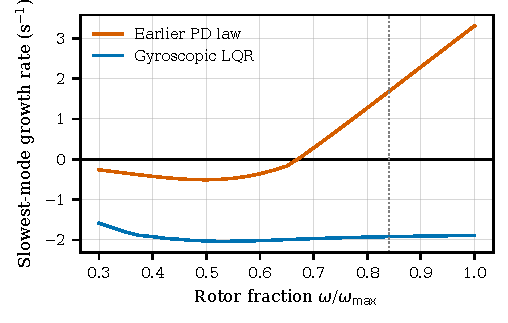
\includegraphics[width=\columnwidth]{lqr.pdf}
\caption{Growth rate of the slowest closed-loop roll/pitch mode on the momentum-vane attitude model \refeq{eq:attplant} at the \SI{30}{\hertz} control period, against rotor fraction.
The earlier PD law is unstable above a rotor fraction of 0.67; the scheduled LQR decays at \SI{1.6}{}--\SI{2.0}{\per\second} throughout.
The dotted line marks hover.}
\label{fig:lqr}
\end{figure}

\section{Verification and Validation}
\label{sec:verification}

\subsection{Test Ladder}

Verification is layered.
The first layer is 40 unit-test modules of pure-tensor checks.
They cover frames, quaternions, fin geometry, the servo, the EDF and battery, the coupled jet's conservation and passivity, rotor reactions, the gyroscopic midpoint, the wind model, intake drag, the contact state machine, crash and reset logic, the IMU, navigation filter and Allan-variance fit, and controller and mission code.
For this review the suite was run on a CPU-only machine with Python~3.12 and PyTorch~2.14, and 433 tests passed, including the ten added with the corrections of \refsec{sec:issues}.
One was skipped because the USD bindings were unavailable.
The second layer is 19 Isaac tests, which require the simulator.
They progress from asset validation, joint axes and single-vane articulation, through unit forces at COPs, vane sweeps, four-vane superposition, spool and gyroscopic precession, wind, contact, a PID hover and a 128-environment API check, to the review-specific regressions.
Those regressions cover net lift and soft contact, the coupled jet in PhysX, thrust-line torque with an offset COM, heading invariance and gyroscopic conservation.
Golden data files pin the vane force sweep, the EDF step reaction and the touchdown cases.
These tests establish that the implementation is consistent with its stated parameters.
They do not establish that those parameters match hardware.

\subsection{Open-Loop Plant Audit in Isaac}

\reftab{tab:audit} reproduces the project's open-loop Isaac audit of the momentum-vane plant~\cite{tang2026rl}.
It was run with scripted vanes and duty and no controller.
Nutation frequency, steady precession under a vane step, yaw acceleration and the throttle-cut momentum exchange all agree with first-principles predictions to within 5\%, at both \SI{120}{\hertz} and \SI{480}{\hertz}.
A regression of Isaac's measured angular acceleration on the model terms over two recorded missions gave coefficients of 0.9--1.03 on the vane and gyroscopic terms and 1.0 on the spool reaction.
For gyroscopic conservation, the review-specific Isaac test kept the rotational-energy drift at or below 0.13\% over two unforced seconds at \SI{480}{\hertz}.
That held with roll and pitch rates of \SI{6.28}{\radian\per\second} and yaw rates up to \SI{\pm40}{\radian\per\second}.
The world angular-momentum error stayed below \SI{1.2e-3}{\newton\metre\second}.

\begin{table}[t]
\caption{Open-Loop Isaac Audit of the Momentum-Vane Plant (Recorded)}
\label{tab:audit}
\centering
\footnotesize
\setlength{\tabcolsep}{3pt}
\begin{tabular}{llll}
\toprule
Test & \SI{120}{\hertz} & \SI{480}{\hertz} & Prediction \\
\midrule
Nutation, neutral vanes & \SI{2.489}{\hertz} & \SI{2.492}{\hertz} & $H/I = \SI{2.48}{\hertz}$ \\
\quad decay rate & \SI{0.019}{\per\second} & \SI{0.018}{\per\second} & \SI{0.018}{\per\second} (\reftab{tab:damping}) \\
Roll step $\to$ precession & \SI{3.70}{\degree\per\second} & \SI{3.72}{\degree\per\second} & \SI{3.9}{\degree\per\second} \\
Yaw step, common mode & \SI{110.6}{\degree\per\second\squared} & \SI{111.1}{\degree\per\second\squared} & \SI{114}{\degree\per\second\squared} \\
Throttle cut in the air & \SI{2242}{\degree\per\second} & \SI{2242}{\degree\per\second} & $\Delta H/I_{zz} = \SI{2233}{\degree\per\second}$ \\
\bottomrule
\end{tabular}
\end{table}

\subsection{Closed-Loop Missions}

The simulator's purpose is to develop guidance that will transfer.
\reftab{tab:missions} lists the recorded Isaac missions that the convex guidance of \refsec{sec:guidance} flew on the momentum-vane mission plant~\cite{tang2026rl}.
All landed inside the gates.
Two later re-flights on the plant with intake momentum drag also landed.
One was a high-energy capture: \SI{0.142}{\metre\per\second} at \SI{0.204}{\metre}.
The other was a gust station-keeping mission: \SI{0.128}{\metre\per\second} at \SI{0.116}{\metre}, after a relaxed hover-hold rule.
Two missions fail for physical rather than algorithmic reasons, and the simulator reproduces why.
Cold in-air starts fail because spooling the rotor moves \SI{0.78}{\newton\metre\second} into a body whose vanes hold about \SI{0.3}{\newton\metre} in yaw.
A \SI{1}{\centi\metre} COM offset fails because it needs about \SI{10}{\degree} of the vanes' \SI{14}{\degree} of usable trim.

\begin{table}[t]
\caption{Recorded Isaac Missions, Convex Guidance on the Momentum-Vane Plant (Warm Rotor)}
\label{tab:missions}
\centering
\footnotesize
\setlength{\tabcolsep}{3pt}
\begin{tabular}{lccc}
\toprule
Mission & Impact & Pad error & Roll/pitch RMS \\
& (\si{\metre\per\second}) & (\si{\metre}) & flight/terminal (\si{\degree\per\second}) \\
\midrule
Default, \SI{18}{\metre} & 0.178 & 0.017 & 0.7 / 0.8 \\
Hop, \SI{3}{\metre} & 0.154 & 0.045 & 5.6 / 3.9 \\
\SI{7}{\metre} offset + crosswind & 0.159 & 0.052 & 6.8 / 2.7 \\
Legacy 6S pack, \SI{8}{\metre} & 0.175 & 0.051 & 7.3 / 1.4 \\
\SI{50}{\metre} start & 0.152 & 0.004 & 0.7 / 0.7 \\
Route: fly-through + hover & 0.152 & 0.098 & 7.3 / 3.3 \\
\SI{50}{\metre}, three hovers, \SI{120}{\second} & 0.148 & 0.063 & 3.8 / 3.2 \\
Wind + noise + COM, \SI{-5}{\metre\per\second} & 0.136 & 0.146 & 9.3 / 4.6 \\
\bottomrule
\end{tabular}
\end{table}

\subsection{Throughput}

On CPU PhysX a single mission vehicle runs at a real-time factor of about 0.75.
The fused navigation filter lowers it to about 0.5.
A ``fast live'' mode reduces headless redraws without touching the physics.
The full-redraw and fast runs of one route produced identical telemetry over all 739 frames.
The physical IMU chain adds 6--12\% of wall time per step at 256 environments.

\section{Discussion: Fidelity Assessment and Open Issues}
\label{sec:discussion}

\subsection{What the Corrected Plant Changes}

Two corrections changed the control problem itself, not just its numbers.
The first is the momentum bound on the vanes.
The second is the removal of the artificial damper.
On the legacy plant, the vanes had 8.47 times their physical authority and the body had 131 times its physical damping.
A proportional-derivative attitude law flew that plant well.
On the momentum plant the same law is unstable above 67\% rotor speed, that is, throughout the flight range (\reffig{fig:lqr}).
The nutation mode sits at $H/I \approx \SI{2.5}{\hertz}$, where the actuator lag exceeds \SI{90}{\degree} of phase, and only saturation and the servo deadband bounded the resulting limit cycles.
A full-state LQR that feeds back both actuator states was needed~\cite{tang2026rl}.
That is the main argument for building the plant from momentum bookkeeping rather than from tuned coefficients.
The tuned plant was not just inaccurate.
It was qualitatively easier than the vehicle it represents.

\subsection{Issues Identified in This Review and Their Status}
\label{sec:issues}

\textbf{(i) Duct Coriolis reaction: corrected.}
The intake momentum drag had been modeled without the Coriolis reaction of the duct flow, which doubled the passive pitch and roll damping.
The mission plant now applies \refeq{eq:coriolis} (\refsec{sec:damping}).
Two tasks remain.
The change should be re-flown in Isaac.
The nozzle station should be confirmed from the CAD, because the configured jet exit at \SI{0.05}{\metre} and the vane COP plane at \SI{0.10}{\metre} disagree.

\textbf{(ii) Sensor timing at the mission step: now reported.}
The IMU and aiding sensors round latency to whole physics substeps and cannot report faster than the physics.
At the \SI{120}{\hertz} mission step, the WTGAHRS1's \SI{5}{\milli\second} latency becomes \SI{8.3}{\milli\second} and its \SI{200}{\hertz} output becomes \SI{120}{\hertz}.
The VN-110E's \SI{2}{\milli\second} latency rounds to zero.
Each sensor model now reports the timing it actually delivers, and missions record it as \texttt{sensor\_timing}.
A run warning flags any latency off by more than 25\%, or any capped output rate.
The rounding itself remains.
Running the sensor chain on a finer internal clock, or interpolating a fractional delay, would remove it.
Until then, timing-sensitive conclusions should be drawn from \SI{480}{\hertz} runs.

\textbf{(iii) Vane-model assumptions.}
Equation \refeq{eq:authority} shows that the model's authority rests on equal streamtube shares and almost complete turning, at a loading of 7.6.
Real vanes in a \SI{90}{\milli\metre} duct may not intercept a full quarter of the jet each, and hub blockage, wall proximity and vane-to-vane interference are absent.
The identification target is therefore the normalized side force $F_\perp/(T/4)$ against $\alpha$, measured on a thrust stand.
The drag fraction $\delta_D$, which sets both the 10.3\% axial loss and the authority, should be measured in the same test.

\textbf{(iv) Environment.}
Gusts are horizontal steps with no vertical component.
A hard-landing analysis needed \SI{1.5}{\metre\per\second\squared} downdrafts offline that the simulator cannot produce.
Ground effect and jet impingement on the pad are not modeled, although the terminal gate sits at \SI{0.8}{\metre}, within two duct diameters of the ground.
The axial intake term is a first-order thrust lapse.
The fan's pressure-rise curve with inflow needs a thrust stand at airspeed.
Body drag acts at the body origin, with no separate aerodynamic center.

\textbf{(v) Actuators and electrical system.}
The motor may brake whenever $d > 0$, and coasts only at $d = 0$.
Whether the real ESC brakes actively during a throttle reduction is firmware-dependent and should be checked.
The servo deadband and lag, the drive stiffness and the rotor inertia are estimates.
Rotor inertia scales every momentum effect in \refsec{sec:reactions}.
All battery coefficients are generic.
The model gives \SI{4.0}{\minute} of hover from a full \SI{5}{\ampere\hour} pack, consistent with \SI{2.1}{\kilo\watt} drawn from \SI{148}{\watt\hour}.
A code comment in the mission service had cited about six minutes; it is corrected.

\textbf{(vi) Documentation drift and result provenance: corrected.}
The scene-setup notes listed the tangential hinge axes that the 2026-09-14 correction replaced.
Two code comments and the IMU notes referred to \SI{480}{\hertz} mission physics, whereas missions run at \SI{120}{\hertz}.
More consequentially, the project README summarized a 7-mission benchmark, landing at 0.146--\SI{0.184}{\metre\per\second}, as a corrected-plant result.
That benchmark was flown on the legacy vane plant, before the mission plant switched to momentum vanes.
The notes and the README now cite the momentum-plant evidence of \reftab{tab:missions}.
The companion manuscript~\cite{tang2026rl} carries the same attribution and should be updated likewise.
The PhysX gravity (\SI{9.81}{\metre\per\second\squared}) and the IMU's standard gravity (\SI{9.80665}{\metre\per\second\squared}) differ by \SI{0.34}{\milli g}, which is negligible against every modeled bias.

\textbf{(vii) Guidance: gap guarded, other items open.}
Lossless convexification is checked, not guaranteed.
The thrust-rate bound could open a convexification gap, which the planner now guards against (\refsec{sec:lcvx}).
Node-to-node thrust alternation appears while the sink envelope binds; a small smoothness weight removes it.
The planner's point-mass model contains no aerodynamics.
Intake momentum drag, \SI{1.26}{\newton} or 4\% of weight in a \SI{4}{\metre\per\second} wind, reaches the plan only through the tracking integrators.
A drag-aware dynamics term, which is linear in velocity and so stays convex, would let the plan anticipate it.
Finally, the measured planning latency on the target flight computer, estimated at 0.2--\SI{0.4}{\second} for a landing plan and 2--\SI{3.5}{\second} for a four-waypoint route, should be validated in Isaac with the latency model before flight.

\subsection{Identification Plan for Transfer}

The open parameters group into a short list of bench experiments, each of which replaces estimates in \reftab{tab:params}.
\begin{itemize}
\item A thrust stand, static and in a wind tunnel or moving cart, for $T(\wrot, V)$, $P(\wrot)$, the inflow thrust lapse and the vane sweep $F_\perp/(T/4)$ and $\delta_D$.
\item A rotor spin-down for $\Ir$ and $Q_a$, since the coast time constant is $\Ir\wrot/Q_a$, and a step response for the current-limited spool.
\item A loaded servo response for $\tau_s$, the slew rate, the deadband and the drive stiffness.
\item A pack discharge at hover power for $E(\mathrm{SOC})$, $R_0$, $R_p$ and $\tau_p$.
\item A static IMU log of at least six hours, with and without the EDF running, for an Allan-variance fit, and a tilted, accelerating rig for the filter gains.
\item A bifilar swing or pendulum test for the inertia tensor and COM, and a free-flight nutation test.
The nutation frequency and decay rate (\SI{2.49}{\hertz} and \SI{0.041}{\per\second} modeled) together check $H$, the inertia and the passive damping.
\end{itemize}

\section{Conclusion}
\label{sec:conclusion}

We have described the physics and simulation implementation behind a sim-to-real study of convex guidance on a jet-vane EDF vehicle.
The force, actuator, electrical, contact and sensor models are bounded by momentum and energy bookkeeping.
Each is tied to its code, its parameter provenance and a regression test.
Offline runs of the production code and recorded Isaac audits support the main claims.
Vane authority is bounded by and reduces to the jet's momentum.
Rotor momentum exchange dominates yaw.
Explicit gyroscopic integration is unusable at the mission step, while the coupled midpoint and Cayley scheme conserves energy and momentum inside PhysX.
The intake dominates low-speed crosswise drag.
The physical passive damping is two orders of magnitude below the tuned value it replaced.
The convex guidance takes its bounds from the same physics.
The rotor's momentum sets the thrust-rate and attitude-slew limits, the battery sets the thrust ceiling, and the vane authority sets the gyroscopic LQR that replaced an attitude law the corrected plant made unstable.
The review corrected the duct's jet-damping bookkeeping, made sensor timing at the mission step explicit, guarded the planner against a convexification gap, and fixed documentation that misattributed results.
It also leaves a concrete list of measurements.
The most important are an Isaac re-flight of the corrected plant and a thrust-stand vane sweep that tests the streamtube assumption on which the model's vane authority rests.

\appendices
\section{Reproducibility}
\label{app:repro}

{\raggedright
The figure scripts are in \texttt{Paper/physics\_simulation/scripts}.
The helper \texttt{plant.py} builds the mission-plant models from \texttt{configs/params}, \texttt{configs/hardware/planned\_8s.yaml} and \texttt{configs/env/mission\_plant.yaml}, merged as mission control merges them.
\texttt{fig\_vane\_force.py}, \texttt{fig\_spool.py}, \texttt{fig\_battery.py}, \texttt{fig\_drag.py}, \texttt{fig\_gyro.py}, \texttt{fig\_imu.py} and \texttt{fig\_lqr.py} produce one figure each, and \texttt{fig\_convex\_plan.py} produces the plan and line-search figures.
Each prints the numbers quoted in the text.
The guidance scripts build the flight computer's vehicle model and controller exactly as the mission runner does.
The printed outputs are saved beside the figures.
The scripts need PyTorch, NumPy, SciPy, PyYAML, Matplotlib and, for the guidance figures, Clarabel, but not Isaac Sim.
The unit tests run with \texttt{pytest} from \texttt{simulation/isaac}, and the Isaac tests with \texttt{apps/run\_single\_test.py}.
\par}

\begin{thebibliography}{99}

\bibitem{acikmese2007}
B.~A\c{c}{\i}kme\c{s}e and S.~R.~Ploen, ``Convex programming approach to powered descent guidance for Mars landing,'' \textit{J. Guid., Control, Dyn.}, vol.~30, no.~5, pp.~1353--1366, 2007.

\bibitem{tang2026rl}
T.~Zijian, ``Reinforcement learning for thrust-vectored fin control of an electric ducted fan VTOL vehicle in simulation,'' manuscript, Minnesota State Univ., Mankato, 2026.

\bibitem{furrer2016rotors}
F.~Furrer, M.~Burri, M.~Achtelik, and R.~Siegwart, ``RotorS---A modular Gazebo MAV simulator framework,'' in \textit{Robot Operating System (ROS): The Complete Reference (Vol.~1)}, A.~Koubaa, Ed. Springer, 2016, pp.~595--625.

\bibitem{song2020flightmare}
Y.~Song, S.~Naji, E.~Kaufmann, A.~Loquercio, and D.~Scaramuzza, ``Flightmare: A flexible quadrotor simulator,'' in \textit{Proc. Conf. Robot Learning (CoRL)}, 2020.

\bibitem{shah2018airsim}
S.~Shah, D.~Dey, C.~Lovett, and A.~Kapoor, ``AirSim: High-fidelity visual and physical simulation for autonomous vehicles,'' in \textit{Field and Service Robotics}. Springer, 2018, pp.~621--635.

\bibitem{panerati2021gym}
J.~Panerati, H.~Zheng, S.~Zhou, J.~Xu, A.~Prorok, and A.~P.~Schoellig, ``Learning to fly---A Gym environment with PyBullet physics for reinforcement learning of multi-agent quadcopter control,'' in \textit{Proc. IEEE/RSJ Int. Conf. Intell. Robots Syst. (IROS)}, 2021.

\bibitem{makoviychuk2021isaac}
V.~Makoviychuk \textit{et al.}, ``Isaac Gym: High performance GPU-based physics simulation for robot learning,'' in \textit{Proc. NeurIPS Datasets and Benchmarks Track}, 2021.

\bibitem{mittal2023orbit}
M.~Mittal \textit{et al.}, ``Orbit: A unified simulation framework for interactive robot learning environments,'' \textit{IEEE Robot. Autom. Lett.}, vol.~8, no.~6, pp.~3740--3747, 2023.

\bibitem{physx2023}
NVIDIA, ``PhysX SDK 5 documentation: Articulations,'' 2023. [Online]. Available: \url{https://nvidia-omniverse.github.io/PhysX/physx/5.5.0/docs/Articulations.html}

\bibitem{sutton2017}
G.~P.~Sutton and O.~Biblarz, \textit{Rocket Propulsion Elements}, 9th~ed. Hoboken, NJ, USA: Wiley, 2017.

\bibitem{luo2018jetvane}
J.~Luo, L.~Zhao, and C.~Cao, ``Research on the thrust vector control via jet vane in rapid turning of vertical launch,'' \textit{J. Mech. Sci. Technol.}, vol.~32, no.~4, pp.~1823--1831, 2018.

\bibitem{johnson2006ducted}
E.~N.~Johnson and M.~A.~Turbe, ``Modeling, control, and flight testing of a small ducted-fan aircraft,'' \textit{J. Guid., Control, Dyn.}, vol.~29, no.~4, pp.~769--779, 2006.

\bibitem{pflimlin2010ducted}
J.-M.~Pflimlin, P.~Binetti, P.~Sou\`eres, T.~Hamel, and D.~Trouchet, ``Modeling and attitude control analysis of a ducted-fan micro aerial vehicle,'' \textit{Control Eng. Pract.}, vol.~18, no.~3, pp.~209--218, 2010.

\bibitem{drela2006qprop}
M.~Drela, ``QPROP formulation,'' MIT Aero \& Astro, 2006. [Online]. Available: \url{https://web.mit.edu/drela/Public/web/qprop/qprop_theory.pdf}

\bibitem{thomson1986}
W.~T.~Thomson, \textit{Introduction to Space Dynamics}. New York, NY, USA: Dover, 1986.

\bibitem{simo1991}
J.~C.~Simo and K.~K.~Wong, ``Unconditionally stable algorithms for rigid body dynamics that exactly preserve energy and momentum,'' \textit{Int. J. Numer. Methods Eng.}, vol.~31, no.~1, pp.~19--52, 1991.

\bibitem{hairer2006}
E.~Hairer, C.~Lubich, and G.~Wanner, \textit{Geometric Numerical Integration}, 2nd~ed. Berlin, Germany: Springer, 2006.

\bibitem{lee2007lie}
T.~Lee, M.~Leok, and N.~H.~McClamroch, ``Lie group variational integrators for the full body problem,'' \textit{Comput. Methods Appl. Mech. Eng.}, vol.~196, pp.~2907--2924, 2007.

\bibitem{chen2006battery}
M.~Chen and G.~A.~Rinc\'on-Mora, ``Accurate electrical battery model capable of predicting runtime and I--V performance,'' \textit{IEEE Trans. Energy Convers.}, vol.~21, no.~2, pp.~504--511, 2006.

\bibitem{plett2015}
G.~L.~Plett, \textit{Battery Management Systems, Volume I: Battery Modeling}. Norwood, MA, USA: Artech House, 2015.

\bibitem{ieee952}
\textit{IEEE Standard Specification Format Guide and Test Procedure for Single-Axis Interferometric Fiber Optic Gyros}, IEEE Std 952-1997, 1998.

\bibitem{elsheimy2008allan}
N.~El-Sheimy, H.~Hou, and X.~Niu, ``Analysis and modeling of inertial sensors using Allan variance,'' \textit{IEEE Trans. Instrum. Meas.}, vol.~57, no.~1, pp.~140--149, 2008.

\bibitem{mahony2008}
R.~Mahony, T.~Hamel, and J.-M.~Pflimlin, ``Nonlinear complementary filters on the special orthogonal group,'' \textit{IEEE Trans. Autom. Control}, vol.~53, no.~5, pp.~1203--1218, 2008.

\bibitem{sola2017}
J.~Sol\`a, ``Quaternion kinematics for the error-state Kalman filter,'' arXiv:1711.02508, 2017.

\bibitem{ardupilot2026ekf3}
ArduPilot Development Team, ``AP\_NavEKF3,'' ArduPilot source, \texttt{libraries/AP\_NavEKF3}, accessed Sep. 2026. [Online]. Available: \url{https://github.com/ArduPilot/ardupilot}

\bibitem{young2011imusim}
A.~D.~Young, M.~J.~Ling, and D.~K.~Arvind, ``IMUSim: A simulation environment for inertial sensing algorithm design and evaluation,'' in \textit{Proc. Int. Conf. Inf. Process. Sensor Netw. (IPSN)}, 2011, pp.~199--210.

\bibitem{hoerner1965}
S.~F.~Hoerner, \textit{Fluid-Dynamic Drag}. Bakersfield, CA, USA: Hoerner Fluid Dynamics, 1965.

\bibitem{acikmese2011lcvx}
B.~A\c{c}{\i}kme\c{s}e and L.~Blackmore, ``Lossless convexification of a class of optimal control problems with non-convex control constraints,'' \textit{Automatica}, vol.~47, no.~2, pp.~341--347, 2011.

\bibitem{blackmore2010mle}
L.~Blackmore, B.~A\c{c}{\i}kme\c{s}e, and D.~P.~Scharf, ``Minimum-landing-error powered-descent guidance for Mars landing using convex optimization,'' \textit{J. Guid., Control, Dyn.}, vol.~33, no.~4, pp.~1161--1171, 2010.

\bibitem{harris2014lcvx}
M.~W.~Harris and B.~A\c{c}{\i}kme\c{s}e, ``Lossless convexification of non-convex optimal control problems for state constrained linear systems,'' \textit{Automatica}, vol.~50, no.~9, pp.~2304--2311, 2014.

\bibitem{malyuta2022convex}
D.~Malyuta, T.~P.~Reynolds, M.~Szmuk, T.~Lew, R.~Bonalli, M.~Pavone, and B.~A\c{c}{\i}kme\c{s}e, ``Convex optimization for trajectory generation: A tutorial on generating dynamically feasible trajectories reliably and efficiently,'' \textit{IEEE Control Syst. Mag.}, vol.~42, no.~5, pp.~40--113, 2022.

\bibitem{goulart2024clarabel}
P.~J.~Goulart and Y.~Chen, ``Clarabel: An interior-point solver for conic programs with quadratic objectives,'' arXiv:2405.12762, 2024.

\bibitem{lee2010geometric}
T.~Lee, M.~Leok, and N.~H.~McClamroch, ``Geometric tracking control of a quadrotor UAV on SE(3),'' in \textit{Proc. IEEE Conf. Decision Control (CDC)}, 2010, pp.~5420--5425.

\bibitem{bryson1975}
A.~E.~Bryson and Y.-C.~Ho, \textit{Applied Optimal Control}. Washington, DC, USA: Hemisphere, 1975.

\bibitem{tao1996}
G.~Tao and P.~V.~Kokotovi\'c, \textit{Adaptive Control of Systems with Actuator and Sensor Nonlinearities}. New York, NY, USA: Wiley, 1996.

\bibitem{kiefer1953}
J.~Kiefer, ``Sequential minimax search for a maximum,'' \textit{Proc. Amer. Math. Soc.}, vol.~4, no.~3, pp.~502--506, 1953.

\end{thebibliography}

\end{document}
